%%%%%%%%%%%%%%%%%%%%%%%%%%%%%%%%%%%%%%%%%%%%%%%%%%%%%%%%%%%%%%%%%%%%%%%%%
%                                                                       %
% ustthesis_test.tex: A template file for usage with ustthesis.cls      %
%                                                                       %
%%%%%%%%%%%%%%%%%%%%%%%%%%%%%%%%%%%%%%%%%%%%%%%%%%%%%%%%%%%%%%%%%%%%%%%%%

\documentclass{ustthesis}


\usepackage{times,amsmath,epsfig}
\DeclareMathOperator*{\argmax}{arg\,max}
\usepackage{graphicx}
\usepackage[linesnumbered,ruled]{algorithm2e}
\usepackage[center]{subfigure}
\usepackage{graphicx}
\usepackage[table]{xcolor}
\usepackage{longtable}
\usepackage{caption}
\captionsetup{labelfont=bf}
\usepackage{amsmath}
\newtheorem{proof}{Proof}
\usepackage[left=2.5cm,top=4.0cm,bottom=2.5cm, right=2.5cm]{geometry}
\usepackage{paralist}
\usepackage{enumitem}
\usepackage[hyphens]{url}
\usepackage{array, booktabs, multirow} % vertical align of table cell content
\newcolumntype{M}[1]{>{\centering\arraybackslash}m{#1}}
\usepackage{adjustbox}
\usepackage{pifont}

\newcommand{\red}[1]{#1}
\newcommand{\tab}[1]{\hspace{3mm}}
\newcommand{\vcenteredinclude}[1]{\begingroup
  \setbox0=\hbox{\includegraphics[height=\baselineskip, keepaspectratio]{#1}}%
\parbox{\wd0}{\box0}\endgroup}


\usepackage[backend=biber, sorting=none]{biblatex}
\addbibresource{ref.bib}
\usepackage[]{hyperref}
\hypersetup{
    linkbordercolor=green,
}

\usepackage{tikz}
\usetikzlibrary{arrows, positioning, shapes, decorations.pathmorphing}
% This is not an official TikZ library. Use at your own risk!

\makeatletter
% alternative latex arrow
\pgfarrowsdeclare{latexnew}{latexnew}
{
  \ifdim\pgfgetarrowoptions{latexnew}=-1pt%
    \pgfutil@tempdima=0.28pt%
    \pgfutil@tempdimb=\pgflinewidth%
    \ifdim\pgfinnerlinewidth>0pt%
      \pgfmathsetlength\pgfutil@tempdimb{.6\pgflinewidth-.4*\pgfinnerlinewidth}%
    \fi%
    \advance\pgfutil@tempdima by.3\pgfutil@tempdimb%
  \else%
    \pgfutil@tempdima=\pgfgetarrowoptions{latexnew}%
    \divide\pgfutil@tempdima by 10%
  \fi%
  \pgfarrowsleftextend{+-1\pgfutil@tempdima}%
  \pgfarrowsrightextend{+9\pgfutil@tempdima}%
}
{
  \ifdim\pgfgetarrowoptions{latexnew}=-1pt%
    \pgfutil@tempdima=0.28pt%
    \pgfutil@tempdimb=\pgflinewidth%
    \ifdim\pgfinnerlinewidth>0pt%
      \pgfmathsetlength\pgfutil@tempdimb{.6\pgflinewidth-.4*\pgfinnerlinewidth}%
    \fi%
    \advance\pgfutil@tempdima by.3\pgfutil@tempdimb%
  \else%
    \pgfutil@tempdima=\pgfgetarrowoptions{latexnew}%
    \divide\pgfutil@tempdima by 10%
    \pgfsetlinewidth{0bp}%
  \fi%
  \pgfpathmoveto{\pgfqpoint{9\pgfutil@tempdima}{0pt}}
  \pgfpathcurveto
  {\pgfqpoint{6.3333\pgfutil@tempdima}{.5\pgfutil@tempdima}}
  {\pgfqpoint{2\pgfutil@tempdima}{2\pgfutil@tempdima}}
  {\pgfqpoint{-1\pgfutil@tempdima}{3.75\pgfutil@tempdima}}
  \pgfpathlineto{\pgfqpoint{-1\pgfutil@tempdima}{-3.75\pgfutil@tempdima}}
  \pgfpathcurveto
  {\pgfqpoint{2\pgfutil@tempdima}{-2\pgfutil@tempdima}}
  {\pgfqpoint{6.3333\pgfutil@tempdima}{-.5\pgfutil@tempdima}}
  {\pgfqpoint{9\pgfutil@tempdima}{0pt}}
  \pgfusepathqfill
}

% alternative latex reversed arrow
\pgfarrowsdeclarereversed{latexnew reversed}{latexnew reversed}{latexnew}{latexnew}

% alternative latex' arrow
\pgfarrowsdeclare{latex'new}{latex'new}
{
  \ifdim\pgfgetarrowoptions{latex'new}=-1pt%
    \pgfutil@tempdima=0.28pt%
    \advance\pgfutil@tempdima by.3\pgflinewidth%
  \else%
    \pgfutil@tempdima=\pgfgetarrowoptions{latex'new}%
    \divide\pgfutil@tempdima by 10%
  \fi%
  \pgfarrowsleftextend{+-4\pgfutil@tempdima}
  \pgfarrowsrightextend{+6\pgfutil@tempdima}
}
{
  \ifdim\pgfgetarrowoptions{latex'new}=-1pt%
    \pgfutil@tempdima=0.28pt%
    \advance\pgfutil@tempdima by.3\pgflinewidth%
  \else%
    \pgfutil@tempdima=\pgfgetarrowoptions{latex'new}%
    \divide\pgfutil@tempdima by 10%
    \pgfsetlinewidth{0bp}%
  \fi%
  \pgfpathmoveto{\pgfqpoint{6\pgfutil@tempdima}{0\pgfutil@tempdima}}
  \pgfpathcurveto
  {\pgfqpoint{3.5\pgfutil@tempdima}{.5\pgfutil@tempdima}}
  {\pgfqpoint{-1\pgfutil@tempdima}{1.5\pgfutil@tempdima}}
  {\pgfqpoint{-4\pgfutil@tempdima}{3.75\pgfutil@tempdima}}
  \pgfpathcurveto
  {\pgfqpoint{-1.5\pgfutil@tempdima}{1\pgfutil@tempdima}}
  {\pgfqpoint{-1.5\pgfutil@tempdima}{-1\pgfutil@tempdima}}
  {\pgfqpoint{-4\pgfutil@tempdima}{-3.75\pgfutil@tempdima}}
  \pgfpathcurveto
  {\pgfqpoint{-1\pgfutil@tempdima}{-1.5\pgfutil@tempdima}}
  {\pgfqpoint{3.5\pgfutil@tempdima}{-.5\pgfutil@tempdima}}
  {\pgfqpoint{6\pgfutil@tempdima}{0\pgfutil@tempdima}}
  \pgfusepathqfill
}

% alternative latex' reversed arrow
\pgfarrowsdeclarereversed{latex'new reversed}{latex'new reversed}{latex'new}{latex'new}

% alternative o arrow
\pgfarrowsdeclare{onew}{onew}
{
  \pgfarrowsleftextend{+-.5\pgflinewidth}
  \ifdim\pgfgetarrowoptions{onew}=-1pt%
    \pgfutil@tempdima=0.4pt%
    \advance\pgfutil@tempdima by.2\pgflinewidth%
    \pgfutil@tempdimb=9\pgfutil@tempdima\advance\pgfutil@tempdimb by.5\pgflinewidth%
    \pgfarrowsrightextend{+\pgfutil@tempdimb}%
  \else%
    \pgfutil@tempdima=\pgfgetarrowoptions{onew}%
    \advance\pgfutil@tempdima by -0.5\pgflinewidth%
    \pgfarrowsrightextend{+\pgfutil@tempdima}%
  \fi%
}
{ 
  \ifdim\pgfgetarrowoptions{onew}=-1pt%
    \pgfutil@tempdima=0.4pt%
    \advance\pgfutil@tempdima by.2\pgflinewidth%
    \pgfutil@tempdimb=0pt%
  \else%
    \pgfutil@tempdima=\pgfgetarrowoptions{onew}%
    \divide\pgfutil@tempdima by 9%
    \pgfutil@tempdimb=0.5\pgflinewidth%
  \fi%
  \pgfsetdash{}{+0pt}
  \pgfpathcircle{\pgfpointadd{\pgfqpoint{4.5\pgfutil@tempdima}{0bp}}%
                             {\pgfqpoint{-\pgfutil@tempdimb}{0bp}}}%
                {4.5\pgfutil@tempdima-\pgfutil@tempdimb}%
  \pgfusepathqstroke
}

% alternative square arrow
\pgfarrowsdeclare{squarenew}{squarenew}
{
 \ifdim\pgfgetarrowoptions{squarenew}=-1pt%
   \pgfutil@tempdima=0.4pt
   \advance\pgfutil@tempdima by.275\pgflinewidth%
   \pgfarrowsleftextend{+-\pgfutil@tempdima}
   \advance\pgfutil@tempdima by.5\pgflinewidth
   \pgfarrowsrightextend{+\pgfutil@tempdima}
 \else%
   \pgfutil@tempdima=\pgfgetarrowoptions{squarenew}%
   \divide\pgfutil@tempdima by 8%
   \pgfarrowsleftextend{+-7\pgfutil@tempdima}%
   \pgfarrowsrightextend{+1\pgfutil@tempdima}%
 \fi%
}
{
 \ifdim\pgfgetarrowoptions{squarenew}=-1pt%
   \pgfutil@tempdima=0.4pt%
   \advance\pgfutil@tempdima by.275\pgflinewidth%
   \pgfutil@tempdimb=0pt%
 \else%
   \pgfutil@tempdima=\pgfgetarrowoptions{squarenew}%   
   \divide\pgfutil@tempdima by 8%
   \pgfutil@tempdimb=0.5\pgflinewidth%
 \fi%
 \pgfsetdash{}{+0pt}
 \pgfsetroundjoin
 \pgfpathmoveto{\pgfpointadd{\pgfqpoint{1\pgfutil@tempdima}{4\pgfutil@tempdima}}
                            {\pgfqpoint{-\pgfutil@tempdimb}{-\pgfutil@tempdimb}}}
 \pgfpathlineto{\pgfpointadd{\pgfqpoint{-7\pgfutil@tempdima}{4\pgfutil@tempdima}}
                            {\pgfqpoint{\pgfutil@tempdimb}{-\pgfutil@tempdimb}}}
 \pgfpathlineto{\pgfpointadd{\pgfqpoint{-7\pgfutil@tempdima}{-4\pgfutil@tempdima}}
                            {\pgfqpoint{\pgfutil@tempdimb}{\pgfutil@tempdimb}}}
 \pgfpathlineto{\pgfpointadd{\pgfqpoint{1\pgfutil@tempdima}{-4\pgfutil@tempdima}}
                            {\pgfqpoint{-\pgfutil@tempdimb}{\pgfutil@tempdimb}}}
 \pgfpathclose
 \pgfusepathqfillstroke
}

% alternative stealth arrow
\pgfarrowsdeclare{stealthnew}{stealthnew}
{
  \ifdim\pgfgetarrowoptions{stealthnew}=-1pt%
    \pgfutil@tempdima=0.28pt%
    \pgfutil@tempdimb=\pgflinewidth%
    \ifdim\pgfinnerlinewidth>0pt%
      \pgfmathsetlength\pgfutil@tempdimb{.6\pgflinewidth-.4*\pgfinnerlinewidth}%
    \fi%
    \advance\pgfutil@tempdima by.3\pgfutil@tempdimb%
  \else%
    \pgfutil@tempdima=\pgfgetarrowoptions{stealthnew}%
    \divide\pgfutil@tempdima by 8%
  \fi%
  \pgfarrowsleftextend{+-3\pgfutil@tempdima}
  \pgfarrowsrightextend{+5\pgfutil@tempdima}
}
{
  \ifdim\pgfgetarrowoptions{stealthnew}=-1pt%
    \pgfutil@tempdima=0.28pt%
    \pgfutil@tempdimb=\pgflinewidth%
    \ifdim\pgfinnerlinewidth>0pt%
      \pgfmathsetlength\pgfutil@tempdimb{.6\pgflinewidth-.4*\pgfinnerlinewidth}%
    \fi%
    \advance\pgfutil@tempdima by.3\pgfutil@tempdimb%
  \else%
    \pgfutil@tempdima=\pgfgetarrowoptions{stealthnew}%
    \divide\pgfutil@tempdima by 8%
    \pgfsetlinewidth{0bp}%
  \fi%
  \pgfpathmoveto{\pgfqpoint{5\pgfutil@tempdima}{0pt}}
  \pgfpathlineto{\pgfqpoint{-3\pgfutil@tempdima}{4\pgfutil@tempdima}}
  \pgfpathlineto{\pgfpointorigin}
  \pgfpathlineto{\pgfqpoint{-3\pgfutil@tempdima}{-4\pgfutil@tempdima}}
  \pgfusepathqfill
}

% alternative stealth reversed arrow
\pgfarrowsdeclarereversed{stealthnew reversed}{stealthnew reversed}{stealthnew}{stealthnew}

% alternative to arrow
\pgfarrowsdeclare{tonew}{tonew}
{
  \ifdim\pgfgetarrowoptions{tonew}=-1pt%
    \pgfutil@tempdima=0.84pt%
    \advance\pgfutil@tempdima by1.3\pgflinewidth%
    \pgfutil@tempdimb=0.21pt%
    \advance\pgfutil@tempdimb by.625\pgflinewidth%
  \else%
    \pgfutil@tempdima=\pgfgetarrowoptions{tonew}%
    \pgfarrowsleftextend{+-0.8\pgfutil@tempdima}%
    \pgfarrowsrightextend{+0.2\pgfutil@tempdima}%
  \fi%
}
{
  \ifdim\pgfgetarrowoptions{tonew}=-1pt%
    \pgfutil@tempdima=0.28pt%
    \advance\pgfutil@tempdima by.3\pgflinewidth%
    \pgfutil@tempdimb=0pt,%
  \else%
    \pgfutil@tempdima=\pgfgetarrowoptions{tonew}%
    \multiply\pgfutil@tempdima by 100%
    \divide\pgfutil@tempdima by 375%
    \pgfutil@tempdimb=0.4\pgflinewidth%
  \fi%
  \pgfsetdash{}{+0pt}
  \pgfsetroundcap
  \pgfsetroundjoin
  \pgfpathmoveto{\pgfpointorigin}
  \pgflineto{\pgfpointadd{\pgfpoint{0.75\pgfutil@tempdima}{0bp}}
                         {\pgfqpoint{-2\pgfutil@tempdimb}{0bp}}}
  \pgfusepathqstroke
  \pgfsetlinewidth{0.8\pgflinewidth}
  \pgfpathmoveto{\pgfpointadd{\pgfqpoint{-3\pgfutil@tempdima}{4\pgfutil@tempdima}}
                             {\pgfqpoint{\pgfutil@tempdimb}{0bp}}}
  \pgfpathcurveto
  {\pgfpointadd{\pgfqpoint{-2.75\pgfutil@tempdima}{2.5\pgfutil@tempdima}}
               {\pgfqpoint{0.5\pgfutil@tempdimb}{0bp}}}
  {\pgfpointadd{\pgfqpoint{0pt}{0.25\pgfutil@tempdima}}
               {\pgfqpoint{-0.5\pgfutil@tempdimb}{0bp}}}
  {\pgfpointadd{\pgfqpoint{0.75\pgfutil@tempdima}{0pt}}
               {\pgfqpoint{-\pgfutil@tempdimb}{0bp}}}
  \pgfpathcurveto
  {\pgfpointadd{\pgfqpoint{0pt}{-0.25\pgfutil@tempdima}}
               {\pgfqpoint{-0.5\pgfutil@tempdimb}{0bp}}}
  {\pgfpointadd{\pgfqpoint{-2.75\pgfutil@tempdima}{-2.5\pgfutil@tempdima}}
               {\pgfqpoint{0.5\pgfutil@tempdimb}{0bp}}}
  {\pgfpointadd{\pgfqpoint{-3\pgfutil@tempdima}{-4\pgfutil@tempdima}}
               {\pgfqpoint{\pgfutil@tempdimb}{0bp}}}
  \pgfusepathqstroke
}

% alias alternative to arrow
\pgfarrowsdeclarealias{<new}{>new}{tonew}{tonew}

\makeatother

% tip length code
\pgfsetarrowoptions{latexnew}{-1pt}
\pgfsetarrowoptions{latex'new}{-1pt}
\pgfsetarrowoptions{onew}{-1pt}
\pgfsetarrowoptions{squarenew}{-1pt}
\pgfsetarrowoptions{stealthnew}{-1pt}
\pgfsetarrowoptions{tonew}{-1pt}
\pgfkeys{/tikz/.cd, arrowhead/.default=-1pt, arrowhead/.code={
  \pgfsetarrowoptions{latexnew}{#1},
  \pgfsetarrowoptions{latex'new}{#1},
  \pgfsetarrowoptions{onew}{#1},
  \pgfsetarrowoptions{squarenew}{#1},
  \pgfsetarrowoptions{stealthnew}{#1},
  \pgfsetarrowoptions{tonew}{#1},
}}




% \usepackage{latexsym}
    % Use the "latexsym" package when encountering the following error:
    %   ! LaTeX Error: Command \??? not provided in base LaTeX2e.
% \usepackage{epsf}
    % Use the "epsf" package for including EPS files.

%%%%%%%%%%%%%%%%%%%%%%%%%%%%%%%%%%%%%%%%%%%%%%%%%%%%%%%%%%%%%%%%%%%%%%%%%
%                                                                       %
% Preambles. DO NOT ERASE THEM. Change to suite your particular purpose.%
%                                                                       %
%%%%%%%%%%%%%%%%%%%%%%%%%%%%%%%%%%%%%%%%%%%%%%%%%%%%%%%%%%%%%%%%%%%%%%%%%

\title{Cardea: A Context-Aware and Interactive Visual Privacy Control Framework}  % Title of the thesis.
\author{Rui~Zheng}     % Author of the thesis.
\degree{\MPhil}             % Degree for which the thesis is.
%% or
%\degree{\PhD}              % Degree for which the thesis is.
\subject{Computer Science and Engineering}      % Subject of the Degree.
\department{Computer Science and Engineering}       % Department to which the thesis
                    % is submitted.
\advisor{Assistant Prof.~Pan.~Hui}     % Supervisor.
\depthead{Prof.~Qiang~Yang}    % department head.
\defencedate{2016}{10}{21}      % \defencedate{year}{month}{day}.

% NOTE:
%   According to the sample shown in the guidelines, page number is
%   placed below the bottom margin.  However, if the author prefers
%   the page number to be printed above the bottom margin, please
%   activate the following command.

% \PNumberAboveBottomMargin

\begin{document}

%%%%%%%%%%%%%%%%%%%%%%%%%%%%%%%%%%%%%%%%%%%%%%%%%%%%%%%%%%%%%%%%%%%%%%%%%
%                                                                       %
% Now the actual Thesis. The order of output MUST be followed:          %
%                                                                       %
%    1) TITLEPAGE                                                       %
%                                                                       %
% The \maketitle command generates the Title page as well as the        %
% Signature page.                                                       %
%                                                                       %
%%%%%%%%%%%%%%%%%%%%%%%%%%%%%%%%%%%%%%%%%%%%%%%%%%%%%%%%%%%%%%%%%%%%%%%%%

\maketitle

%%%%%%%%%%%%%%%%%%%%%%%%%%%%%%%%%%%%%%%%%%%%%%%%%%%%%%%%%%%%%%%%%%%%%%%%%
%                                                                       %
%     2) DEDICATION (Optional)                                          %
%                                                                       %
% The \dedication and \enddedication commands are optional. If          %
% specified it generates a page for dedication.                         %
%
%%%%%%%%%%%%%%%%%%%%%%%%%%%%%%%%%%%%%%%%%%%%%%%%%%%%%%%%%%%%%%%%%%%%%%%%%

% \dedication
% This is an optional section.
% \enddedication

%%%%%%%%%%%%%%%%%%%%%%%%%%%%%%%%%%%%%%%%%%%%%%%%%%%%%%%%%%%%%%%%%%%%%%%%%
%                                                                       %
%     3) ACKNOWLEDGMENTS                                                %
%                                                                       %
% \acknowledgments and \endacknowledgments defines the                  %
% Acknowledgments of the author of the Thesis.                          %
%                                                                       %
%%%%%%%%%%%%%%%%%%%%%%%%%%%%%%%%%%%%%%%%%%%%%%%%%%%%%%%%%%%%%%%%%%%%%%%%%

\acknowledgments

First I would like to thank my family for their unconditional support during the past three years. It is their optimistic attitudes as well as patience that helped me walk across all the troubled water among the years.

I would also like to express my deepest gratitude to my advisor Prof. Pan Hui for his support, guidance and encouragement, without which this thesis would not have been possible.

Special thanks to Jiayu Su, it was a great pleasure to collaborate with her in the past year and I learned a lot from the collaboration. Same thanks gives to Dr. Tongfeng Weng for the enjoyable collaboration on random walks. Other than that, I would like to thank Haris Mughees and Hamza Zia, for countless times we happily talked about everything and I was always surprised by their knowledge, passion as well as determination.

Thanks also goes to all the members in Symlab family. I am fortunate to know so many wonderful people and work as college with them. They have helped me a lot in many aspects from daily life to research. Many thanks to Mr. Issac Ma and Mrs. Connie Lau for their administration work.

Last but not least, I would like to thank Prof. Dit-Yan Yeung and Prof. Chi-Keung Tang. It was great fun to take their courses, which guided me to find my interests and thesis topic. I deeply admire the strong sense of responsibility they have on both lecturing as well as supervision of their students. Their research attitudes and hard working will keep motivating me in my future endeavors.

\endacknowledgments


%%%%%%%%%%%%%%%%%%%%%%%%%%%%%%%%%%%%%%%%%%%%%%%%%%%%%%%%%%%%%%%%%%%%%%%%%
%                                                                       %
%     4) TABLE OF CONTENTS                                              %
%                                                                       %
%%%%%%%%%%%%%%%%%%%%%%%%%%%%%%%%%%%%%%%%%%%%%%%%%%%%%%%%%%%%%%%%%%%%%%%%%

\tableofcontents

%%%%%%%%%%%%%%%%%%%%%%%%%%%%%%%%%%%%%%%%%%%%%%%%%%%%%%%%%%%%%%%%%%%%%%%%%
%                                                                       %
%     5) LIST OF FIGURES (If Any)                                       %
%                                                                       %
%%%%%%%%%%%%%%%%%%%%%%%%%%%%%%%%%%%%%%%%%%%%%%%%%%%%%%%%%%%%%%%%%%%%%%%%%

\listoffigures

%%%%%%%%%%%%%%%%%%%%%%%%%%%%%%%%%%%%%%%%%%%%%%%%%%%%%%%%%%%%%%%%%%%%%%%%%
%                                                                       %
%     6) LIST OF TABLES (If Any)
%                                                                       %
%%%%%%%%%%%%%%%%%%%%%%%%%%%%%%%%%%%%%%%%%%%%%%%%%%%%%%%%%%%%%%%%%%%%%%%%%

\listoftables

%%%%%%%%%%%%%%%%%%%%%%%%%%%%%%%%%%%%%%%%%%%%%%%%%%%%%%%%%%%%%%%%%%%%%%%%%
%                                                                       %
%     7) ABSTRACT                                                       %
%                                                                       %
% \abstract and \endabstract are used to define a short Abstract for    %
% the Thesis.                                                           %
%                                                                       %
%%%%%%%%%%%%%%%%%%%%%%%%%%%%%%%%%%%%%%%%%%%%%%%%%%%%%%%%%%%%%%%%%%%%%%%%%

\begin{abstract}

The growing popularity of mobile and wearable devices with built–in cameras, the bright prospect of camera related applications such as augmented reality and life–logging system, the increased ease of taking and sharing photos, along with advances in computer vision techniques, have greatly facilitated people’s lives in many aspects, but inevitably raised people’s concerns about visual privacy at the same time.

Motivated by the finding that people’s privacy concerns are influenced by the context, in this thesis, we propose Cardea, a context--aware and interactive visual privacy control framework that enforces privacy policies according to people’s privacy preferences. The framework provides people with fine–grained visual privacy control using:
\begin{inparaenum}[\itshape i\itshape)]
\item personal privacy profiles, with which people can define their context--dependent privacy preferences;
\item natural visual indicators: face features, for devices to automatically locate individuals who request privacy protection;
\item hand gestures, for people to temporarily update and flexibly inform cameras of their privacy preferences.
\end{inparaenum}
Benefited from recent progresses in face and object recognition, Cardea offers a way for context--dependent privacy control in a natural and flexible manner, which differs from tag and marker based systems. We design and implement the framework consisting of Android client app and cloud control server, with convolutional neural networks as core of the image processing module. Our evaluation results confirm such framework is practical and effective, showing promising future for context--aware visual privacy control on mobile and wearable devices.

\end{abstract}


%%%%%%%%%%%%%%%%%%%%%%%%%%%%%%%%%%%%%%%%%%%%%%%%%%%%%%%%%%%%%%%%%%%%%%%%%
%                                                                       %
%     8) The Actual Contents                                            %
%                                                                       %
% The command \chapters MUST BE USED to ensure that the entire content  %
% of the Thesis is double-spaced (in version 1.0).                      %
%                                                                       %
% However, in version 2.0, \chapters will be automatically added in     %
% the beginning of the first chapter.                                   %
%                                                                       %
%%%%%%%%%%%%%%%%%%%%%%%%%%%%%%%%%%%%%%%%%%%%%%%%%%%%%%%%%%%%%%%%%%%%%%%%%

%%\chapters         % Not necessary with ustthesis.cls (v2.0).

%%%%%%%%%%%%%%%%%%%%%%%%%%%%%%%%%%%%%%%%%%%%%%%%%%%%%%%%%%%%%%%%%%%%%%%%%
%                                                                       %
% Each chapter is defined via the \chapter command. The usual sectional %
% commands of LaTeX are also available.                                 %
%                                                                       %
%%%%%%%%%%%%%%%%%%%%%%%%%%%%%%%%%%%%%%%%%%%%%%%%%%%%%%%%%%%%%%%%%%%%%%%%%

% \chapter{Introduction}\label{sec-introduction}

The concern about visual privacy has been growing in last decade with increasing adoption of video surveillance systems for security reasons. The statistics shows there are 125 video surveillance cameras per thousand people in U.S. by 2014~\cite{links:numofsurv}. Momentum of new technologies such as the Internet of Things (IOT) will keep driving global video surveillance market in following years, which will raise more privacy concerns.

Other than closed-circuit television (CCTV) surveillance systems for security reasons, handheld devices such as camera phones are also used extensively for the recording of meaningful life moments. Recently, coming with the explosion of products in augmented reality (e.g., Google Glass), robotics (e.g., iRobot Create platform), and gaming (e.g., Kinect), is more and more cameras being embedded in these platforms for the enhancement of life experiences. The trend of embedding cameras, especially in wearables, will keep growing, an example of which is smart contact lens~\cite{links:eyecontact}. However, the ubiquitous presence of cameras, the ease of taking photos and recording videos, along with ``always on'' and ``non overt act'' features threaten individuals to have private or anonymous social lives, raising people's concerns of visual privacy.

More specifically, photos and videos captured without getting permissions from bystanders, and then uploaded to social networking sites, can be accessed by everyone online, potentially leading to invasion of privacy. Malicious applications on the device may also inadvertently leak captured media data~\cite{links:appleakspriv}.

Benefited from research breakthroughs from deep learning community~\cite{Goodfellow-et-al-2016-Book}, current vision perception systems are advancing fast in their capabilities of understanding image and video contents~\cite{links:awesomedeepvision}. Nowadays, recognition technologies can link images to specific people~\cite{taigman2014deepface,sun2015deepid3,schroff2015facenet}, places~\cite{weyand2016planet}, and general objects~\cite{russakovsky2015imagenet}, making what previously unsearchable now searchable~\cite{acquisti2014face}, thus reveal far more private information than expected.

Both legal and technical measures have been proposed to resolve visual privacy concerns. For instance, Google Glass is banned at places such as banks, hospitals, and bars~\cite{links:glassbanned}. However, prohibition of cameras usage does not resolve the issue fundamentally, instead it may intrude people's rights to capture happy moments. As a result, there are growing needs to design technical solutions to protect individuals' visual privacy in a world with pervasive cameras. Technical solutions that have been proposed so far are still limited, in the way that they are mostly based on static policies, thus users can not flexibly express their individualized privacy preferences based on surrounding contexts when they are captured. Moreover, previous works require users to wear visual markers such as hats~\cite{schiff2009respectful} for the detection of interested persons, or clip tags such as QR codes~\cite{bo2014privacy,roesner2014world} for the fetching of privacy polices. Despite technical feasibilities of these approaches, the extra need of setting up markers/tags and the resulting aesthetically unpleasant appearance will hinder users' willingness to adopt these solutions.

Therefore, the motivation of this thesis is to seek a more natural, user–friendly, flexible, and fine-grained mechanism for people to express, modify, and control their individualized privacy preferences. Under this guideline, we propose Cardea, a context-aware and interactive visual privacy control framework, which lets individuals control their visual privacies through:
\begin{inparaenum}[\itshape i\itshape)]
\item personal privacy profiles, with which people can define their context–dependent privacy preferences;
\item different visual indicators: face features and tags, for devices to automatically locates individuals who request privacy protection;
\item hand gestures, for people to temporarily update and flexibly inform cameras of their privacy preferences.
\end{inparaenum}
When using Cardea, the device will automatically compute context factors, compare them with people’s privacy profiles, and finally enforce privacy policies conforming to people’s privacy preferences. To our knowledge, this is one of the pioneering works that leverages deep learning models, more specifically convolutional neural networks (CNN)~\cite{lecun1998gradient}, to enable visual privacy control in a context-specific and interactive manner.

The rest of the thesis is organized as follows: We first review and discuss related works on visual privacy control in Chapter 2. Following that we introduce convolutional neural networks, the core of Cardea's image processing module, and their applications on related computer vision problems. We then give details about the design, implementation and evaluation of Cardea in Chapter 4. Finally, we share our thoughts on possible future work and conclude the thesis in Chapter 5.

\newpage

% \chapter{Related Works}\label{sec-related}

\section{User Studies}





%% use table + adjustbox
% \begin{table}[ht]
  % \centering
  % \begin{adjustbox}{width=1.2\textwidth, center=\textwidth}
  % \begin{tabular}{M{1cm}|M{1cm}|M{2.1cm}|M{1.5cm}|M{1.5cm}|M{2.1cm}|M{1.5cm}|M{2.1cm}|M{1cm}|M{1.5cm}}

%% or use longtable
\setlength\LTleft{-1.7cm}
\begin{longtable}{M{1cm}|M{1.2cm}|M{2.1cm}|M{1.5cm}|M{1.5cm}|M{2.1cm}|M{1.5cm}|M{2.1cm}|M{1cm}|M{1.5cm}}
    \toprule \hline
    \multirow{2}{1cm}[-0.5em]{year} & \multirow{2}{1.2cm}[-0.5em]{\centering privacy survey} & \multicolumn{2}{c|}{problem setting} & \multicolumn{2}{c|}{technical solution} & \multicolumn{2}{c|}{enforcement time} & \multicolumn{2}{c}{privacy object}\\
    \cline{3-10}
    & & video surveillance & mobile cameras & computer vision & cryptography & in-situ / run time & access / distribution & user & bystander\\
    \hline
    \endhead

    \rowcolor{lightgray}\multicolumn{10}{p{19.5cm}}{I-Pic: A Platform for Privacy-Compliant Image Capture~\cite{aditya2016pic}}\\
    2016 & \ding{51} & & \ding{51} & \ding{51} & \ding{51} & \ding{51} & & & \ding{51} \\
    \cline{1-10}
    \multicolumn{10}{p{19.5cm}}{Recent work which allows people to broadcast their privacy preferences and appearance information to nearby devices through BLE. These preferences are based on social context.}\\
    \hline

    \rowcolor{lightgray}\multicolumn{10}{p{19.5cm}}{What You Mark is What Apps See~\cite{raval2016you}}\\
    2016 & & & \ding{51} & \ding{51} & & \ding{51} & \ding{51} & \ding{51} & \\
    \cline{1-10}
    \multicolumn{10}{p{19.5cm}}{Propose a system that give users control to mark secure regions for third-party applications. It is implemented within Android camera subsystem.}\\
    \hline

    \rowcolor{lightgray}\multicolumn{10}{p{19.5cm}}{Sensitive Lifelogs: A Privacy Analysis of Photos from Wearable Cameras~\cite{hoyle2015sensitive}}\\
    2015 & \ding{51} & & \ding{51} & & & & & & \\
    \cline{1-10}
    \multicolumn{10}{p{19.5cm}}{Analyze the photos collected in~\cite{hoyle2014privacy}, seeking to understand what makes a photo private and what participants said about their images.}\\
    \hline

    \rowcolor{lightgray}\multicolumn{10}{p{19.5cm}}{Screenavoider: Protecting Computer Screens from Ubiquitous Cameras~\cite{korayem2014screenavoider}}\\
    2014 & & & \ding{51} & \ding{51} & & \ding{51} & \ding{51} & \ding{51} & \\
    \cline{1-10}
    \multicolumn{10}{p{19.5cm}}{Present a framework that controls the collection and disclosure of lifelogging datasets which contain computer screens and possible sensitive contents.}\\
    \hline

    \rowcolor{lightgray}\multicolumn{10}{p{19.5cm}}{PlaceAvoider: Steering First-Person Cameras away from Sensitive Spaces~\cite{templeman2014placeavoider}}\\
    2014 & & & \ding{51} & \ding{51} & & \ding{51} & \ding{51} & \ding{51} & \\
    \cline{1-10}
    \multicolumn{10}{p{19.5cm}}{Introduce a prototype for owners of first-person cameras to 'blacklist' sensitive places (like bathrooms and bedrooms).}\\
    \hline

    \rowcolor{lightgray}\multicolumn{10}{p{19.5cm}}{Privacy.Tag: Privacy Concern Expressed and Respected~\cite{bo2014privacy}}\\
    2014 & & & \ding{51} & \ding{51} & \ding{51} & & \ding{51} & & \ding{51} \\
    \cline{1-10}
    \multicolumn{10}{p{19.5cm}}{Propose using QR code as privacy tag to link an individual with his photo sharing preferences. These preferences are based on web domains.}\\
    \hline

    \rowcolor{lightgray}\multicolumn{10}{p{19.5cm}}{Privacy Behaviors of Lifeloggers using Wearable Cameras~\cite{hoyle2014privacy}}\\
    2014 & \ding{51} & & \ding{51} & & & \ding{51} & \ding{51} & \ding{51} & \ding{51} \\
    \cline{1-10}
    \multicolumn{10}{p{19.5cm}}{Conducted an \emph{in situ} user study on privacy behaviors of 36 participants who wore lifelogging devices for a week.}\\
    \hline

    \rowcolor{lightgray}\multicolumn{10}{p{19.5cm}}{Courteous Glass~\cite{jung2014courteous}}\\
    2014 & & & \ding{51} & \ding{51} & & \ding{51} & & & \ding{51} \\
    \cline{1-10}
    \multicolumn{10}{p{19.5cm}}{Wearable camera integrated with a FIR (far-infrared) imagers that turns off recording when new persons or specific gestures are detected.}\\
    \hline

    \rowcolor{lightgray}\multicolumn{10}{p{19.5cm}}{World-Driven Access Control for Continuous Sensing~\cite{roesner2014world}}\\
    2014 & & & \ding{51} & \ding{51} & & \ding{51} & \ding{51} & \ding{51} & \\
    \cline{1-10}
    \multicolumn{10}{p{19.5cm}}{Propose a general framework that allows objects to explicitly specify its access policies. Policy triggers can be visual indicators or anything that can be detected in other research works.}\\
    \hline

    \rowcolor{lightgray}\multicolumn{10}{p{19.5cm}}{In Situ with Bystanders of Augmented Reality Glasses: Perspectives on Recording and Privacy-Mediating Technologies~\cite{denning2014situ}}\\
    2014 & \ding{51} & & \ding{51} & & & \ding{51} & \ding{51} & \ding{51} & \ding{51} \\
    \cline{1-10}
    \multicolumn{10}{p{19.5cm}}{Investigate the privacy perspectives of individuals when they are bystanders around AR devices. Conducted 12 field sessions in caf\'es and interviewed 31 bystanders regarding their reactions to a co-located AR device.}\\
    \hline

    \rowcolor{lightgray}\multicolumn{10}{p{19.5cm}}{A Scanner Darkly: Protecting User Privacy From Perceptual Applications~\cite{jana2013scanner}}\\
    2013 & & \ding{51} & \ding{51} & \ding{51} & & \ding{51} & \ding{51} & \ding{51} & \\
    \cline{1-10}
    \multicolumn{10}{p{19.5cm}}{Perceptual applications can only access transformed objects such as sketches, faces, etc.}\\
    \hline

    \rowcolor{lightgray}\multicolumn{10}{p{19.5cm}}{Enabling Fine-Grained Permissions for Augmented Reality Applications With Recognizers~\cite{jana2013enabling}}\\
    2013 & & & \ding{51} & \ding{51} & & \ding{51} & & \ding{51} & \\
    \cline{1-10}
    \multicolumn{10}{p{19.5cm}}{Third party AR applications can only access high-level objects such as Skeleton, Hand Position, etc.}\\
    \hline

    \rowcolor{lightgray}\multicolumn{10}{p{19.5cm}}{PriSurv: Privacy Protected Video Surveillance System Using Adaptive Visual Abstaction~\cite{chinomi2008prisurv}}\\
    2008 & & \ding{51} & & \ding{51} & & & \ding{51} & \ding{51} & \ding{51} \\
    \cline{1-10}
    \multicolumn{10}{p{19.5cm}}{Propose a privacy control mechanism for surveillance videos based on closeness between content objects and content viewers. RFID tags are used to improve the detection of people in videos.}\\
    \hline

    \rowcolor{lightgray}\multicolumn{10}{p{19.5cm}}{Respectful Cameras: Detecting Visual Markers in Real-Time to Address Privacy Concerns~\cite{schiff2009respectful}}\\
    2007 & & \ding{51} & & \ding{51} & & & \ding{51} & \ding{51} & \ding{51} \\
    \cline{1-10}
    \multicolumn{10}{p{19.5cm}}{A video surveillance system that allows people who wish to remain anonymous wear colored markers such as hats or vests, and their faces will be blurred.}\\
    \hline

    \rowcolor{lightgray}\multicolumn{10}{p{19.5cm}}{Privacy Management for Portable Recording Devices~\cite{halderman2004privacy}}\\
    2004 & & & \ding{51} & & \ding{51} & & \ding{51} & \ding{51} & \\
    \cline{1-10}
    \multicolumn{10}{p{19.5cm}}{Propose an approach that closed closed devices can encrypt data together during recording utilizing short range wireless communication to exchange public keys and negotiate encryption key. Only by obtaining all of permissions from people who encrypt the recording can one decrypts it.}\\

    \hline \bottomrule

    \caption{Mobile cameras include cameras in smartphones, AR, VR, lifelogging and other wearable devices. Computer vision methods may be assisted with extra sensors such as RFID tags~\cite{chinomi2008prisurv}, FIR imagers~\cite{jung2014courteous}. There are other factors like implementation layer (app level or os level) that are not listed due to space limitation.}
    \label{tbl-relatedworks}
%% if use table + adjustbox
  % \end{tabular}
  % \end{adjustbox}
% \end{table}

\end{longtable}



\section{Proposed Solutions}

\section{Challenges}

\newpage

% \chapter{Convolutional Neural Networks}\label{sec-cnn}

\section{Deep Learning}

Deep learning~\cite{lecun2015deep, Goodfellow-et-al-2016-Book} is part of a broader family of machine learning methods that focus on representation learning. Unlike rule based methods used in early days of artificial intelligence, deep learning targets at tasks that are easy for people to perform but hard for people to describe formally---problems that we solve intuitively. Former methods have proved success in problems that can be completely described by a very brief list of completely formal rules, thus easily provided ahead of time by the programmer. That led to the defeat of world chess champion Garry Kasparov by IBM's Deep Blue chess-playing system in 1997~\cite{hsu2002behind}. However, rule based or knowledge based methods fail at intuitive tasks such as recognizing objects or speech. The reason behind this inability is because these tasks require immense amount of knowledge about the world, and much of this knowledge is subjective and intuitive, thus difficult to articulate in a formal way. The difficulties faced by AI systems relying on hard-coded knowledge suggest that AI systems need the ability to acquire their own knowledge, by extracting patterns from raw data, just like how human learns from experiences. This capability is known as machine learning. It does not take long for people to realize that performance of machine learning algorithms depends heavily on the representation of data fed into these algorithms. Under a good representation, factors of variation can be disentangled and non important factors will be discarded. People used to put lots of efforts on hand designing features to get a good representation for every domain specific problem. Unfortunately seeking a good representation for a problem can be as difficult as solving the problem itself. Deep learning solves this central problem in representation learning by introducing representations that are expressed in terms of other, simpler representations. Deep learning allows the computer to build complex concepts out of simpler concepts, thus achieves great power and flexibility by representing the world as a nested hierarchy of concepts. Fig~\ref{fig:ch3-dlrelation} shows a hierarchy relation from AI to deep learning.

\begin{figure}[t]
    \centering
    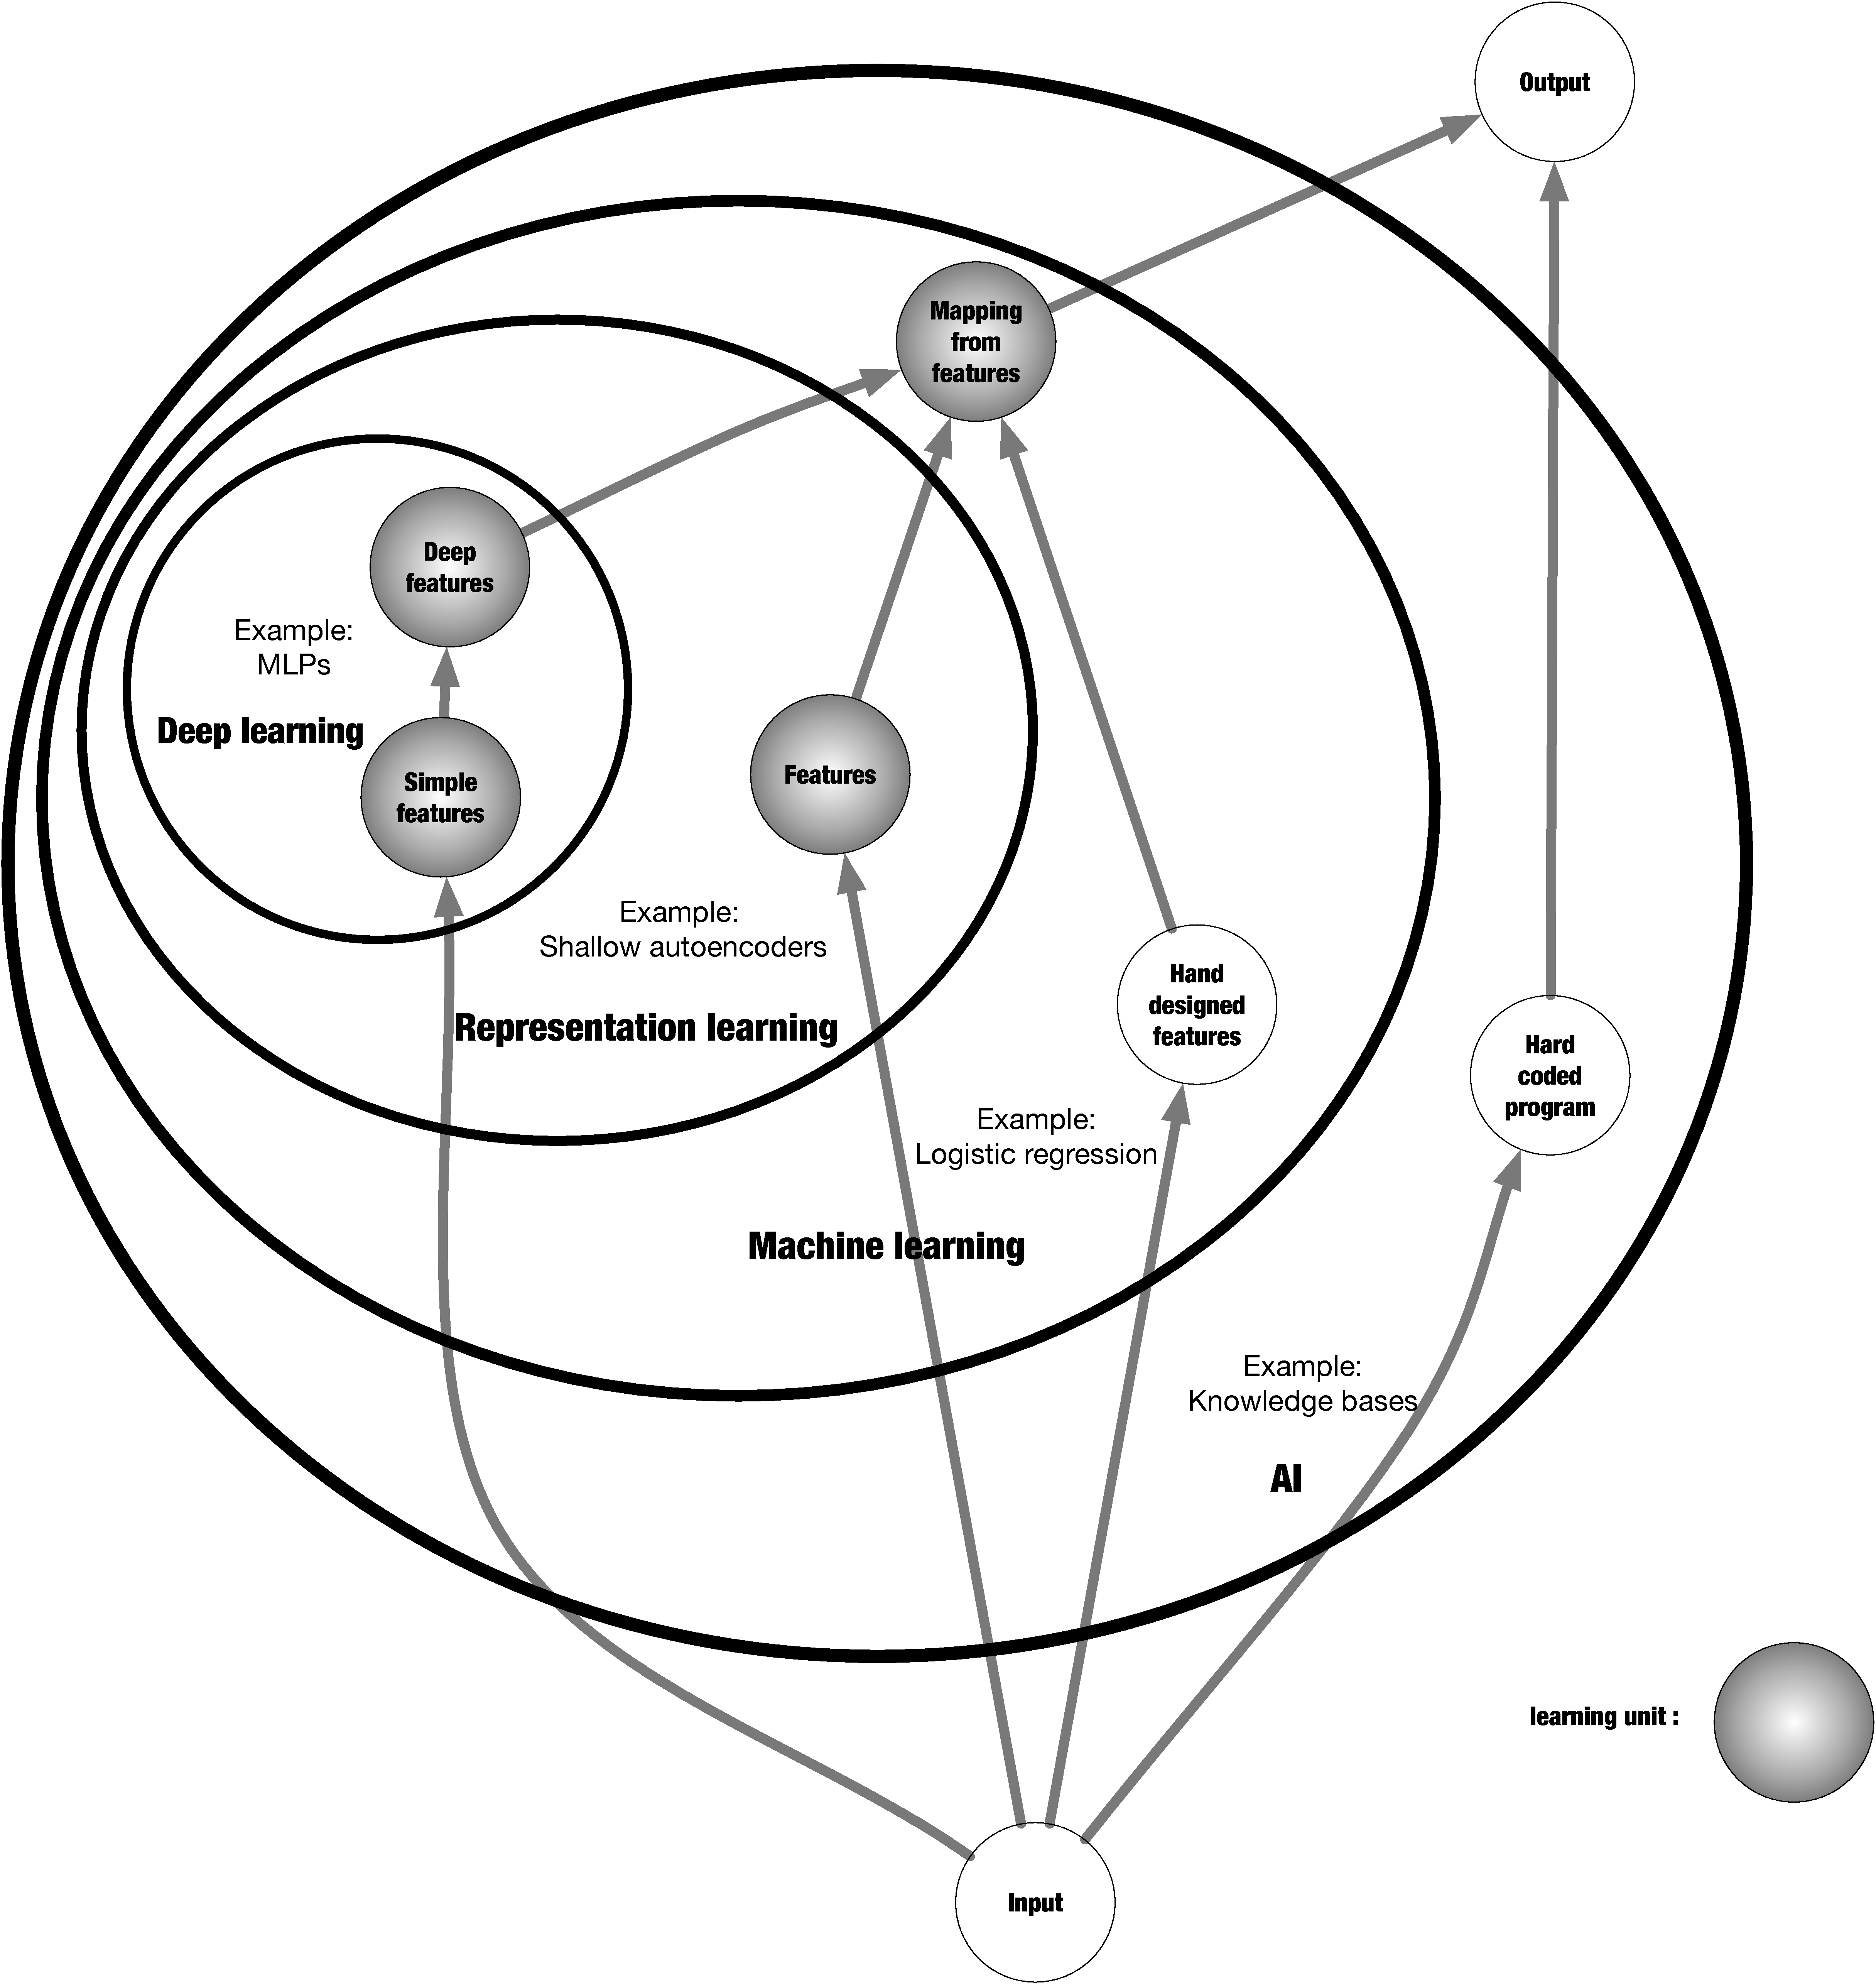
\includegraphics[width=0.5\textwidth]{figure/ch3-dlrelation.pdf}
    \caption{Venn diagram showing relations between deep learning, representation learning, machine learning, and AI. An example and work flow are also included for each section.}
    \label{fig:ch3-dlrelation}
\end{figure}

\subsection{Three Waves}
Deep learning has been rebranded many times under different names, only recently become well known as "deep learning". Broadly speaking, there have been three waves of development of deep learning: in 1940s-1960s known as \emph{cybernetics}~\cite{hebb2005organization, rosenblatt1958perceptron}, in 1980s-1990s known as \emph{connectionism}~\cite{rumelhart1985learning}, and the current resurgence starts from 2006~\cite{Hinton:2006:FLA,hinton2006reducing,Bengio07greedylayer-wise}. These three waves witness the evolving from simple perceptron, to distributed representation and stochastic gradient descent algorithm, and finally to today's various deep structures. The resurgence of deep learning benefits from the facts: computers are faster, datasets are bigger and a good initialization of model parameters. Faster computers make it possible to train deeper models, bigger datasets relieve deep models from overfitting, and enable them to learn more meaningful mid-level features that are more generalizable, and a good initialization through layer wise pretraining provides a proper prior and makes supervised training on later stages much easier.

Since the early stage of deep learning, neuroscience is regarded as an important source of inspiration. However, it is no longer a predominant guide for the field because we simply do not have enough information about the brain to use it as a guide. It is seemed as a more general principle of learning multiple levels of composition, which can be applied in machine learning frameworks that are not necessarily neurally inspired.


\subsection{Breakthroughs}
We highlight some of the breakthroughs brought by deep learning in recent years:
\begin{itemize}
\item In the ImageNet Large-Scale Visual Recognition Challenge (ILSVRC) 2012, a convolutional neuron network won this challenge for the first time and by a wide margin, bringing down the state-of-the-art top-5 error rate from 26.1\% to 15.3\%~\cite{krizhevsky2012imagenet}, since then the top-5 error rate keeps dropping down each year~\cite{SimonyanZ14a, szegedy2015going} and in last year dropped to 3.6\% using deep residual network (ResNet)~\cite{kmhresnet15}. Deep networks also had spectacular successes for pedestrian detection and image segmentation~\cite{sermanet2013pedestrian,farabet2013learning,couprie2013indoor} and yield superhuman performance in traffic sign classification~\cite{cirecsan2012multi}.
\item In March, Google DeepMind's AlphaGo defeated world champion Lee Sedol using deep reinforcement learning~\cite{silver2016mastering,links:alphagovslee}. Prior to that, they also showed that a deep reinforcement system is capable of learning to play Atari video games and reaching human-level performance on many tasks~\cite{mnih2013playing}.
\item The application of deep learning on other fields such as speech recognition~\cite{dahl2010phone, deng2010binary, hinton2012deep} and machine translation~\cite{sutskever2014sequence, bahdanau2014neural} all lead to great successes. The past years surfaced many new trends such as generative adversarial networks, neural Turing machines etc~\cite{goodfellow2014generative, radford2015unsupervised, graves2014neural, xu2015show, links:olah2016attention}. The years ahead are full of challenges and opportunities to improve deep learning even further and bring it to new frontiers.
\end{itemize}



\subsection{Artificial Neural Networks}

\subsubsection{A Single Neuron}
\begin{figure}[t]
    \centering
    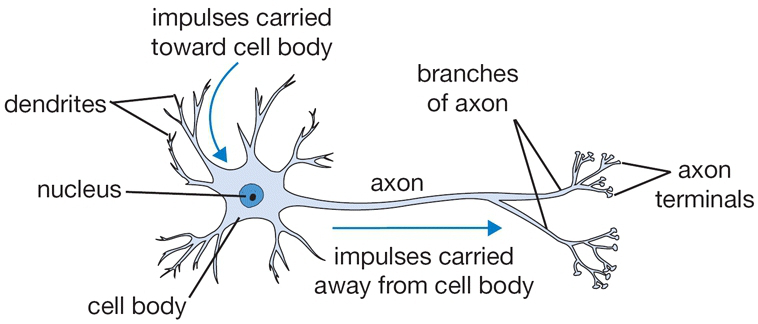
\includegraphics[width=0.45\textwidth]{figure/ch3-bioneuron.png}
    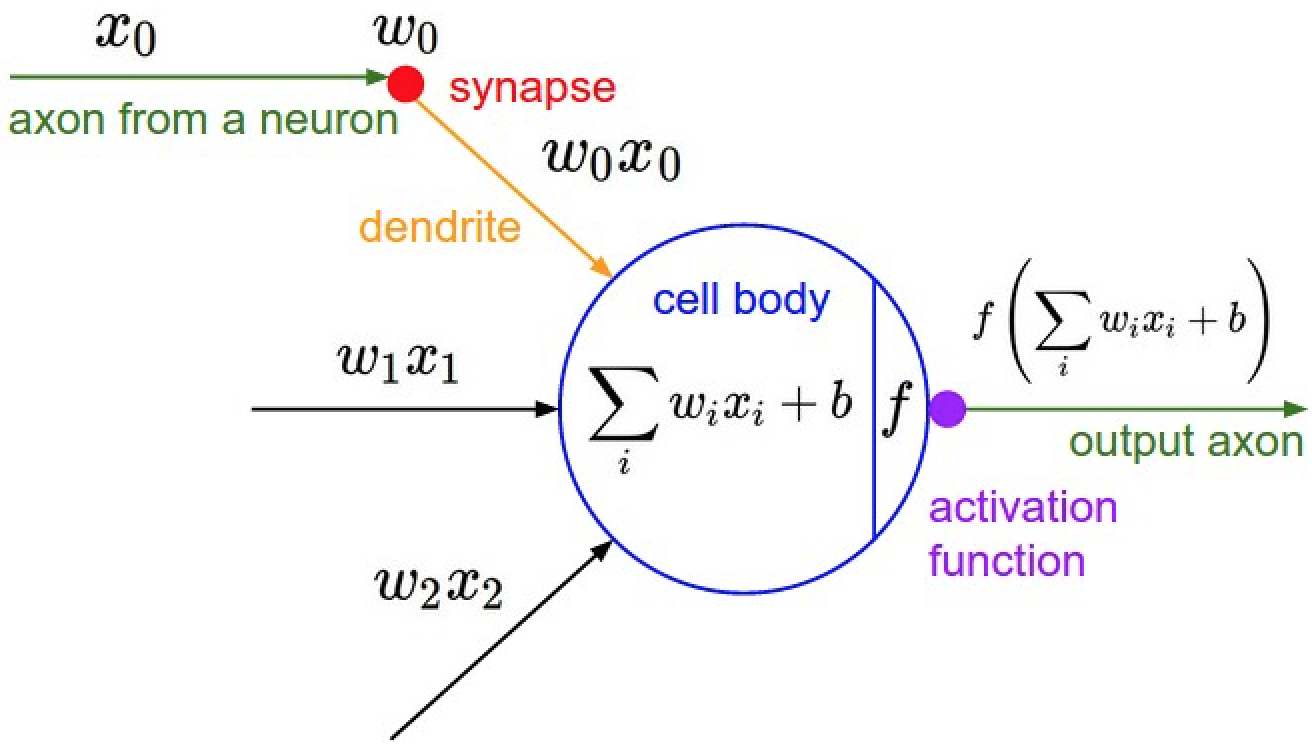
\includegraphics[width=0.45\textwidth]{figure/ch3-compneuron.png}
    \caption{A  cartoon drawing of a biological neuron (left) and its mathematical model (right). Photo taken from \emph{Module1: Neural Networks} in~\cite{links:cs231n}}
    \label{fig:ch3-neuron}
\end{figure}


Fig~\ref{fig:ch3-neuron} shows how to coarsely model a biological neuron: Each neuron receives input signals from its dendrites and produces output signals along its (single) axon. The axon eventually branches out and connects via synapses to dendrites of other neurons. In the basic model, the dendrites carry the signal to the cell body where they all get summed. If the final sum is above a certain threshold, the neuron can fire, sending a spike along its axon. In the computational model, we assume that the precise timings of the spikes do not matter, and that only the frequency of the firing communicates information. Based on this rate code interpretation, we model the firing rate of the neuron with an activation function $f$, which represents the frequency of the spikes along the axon. Historically, a common choice of activation function is the sigmoid function $\sigma$, since it takes a real-valued input (the signal strength after the sum) and squashes it to range between 0 and 1. Hereafter in this thesis, we will take standard naming convention and refer a hidden unit as a computational neuron.

\subsubsection{Activations}

\begin{figure}[!htbp]
    \centering
    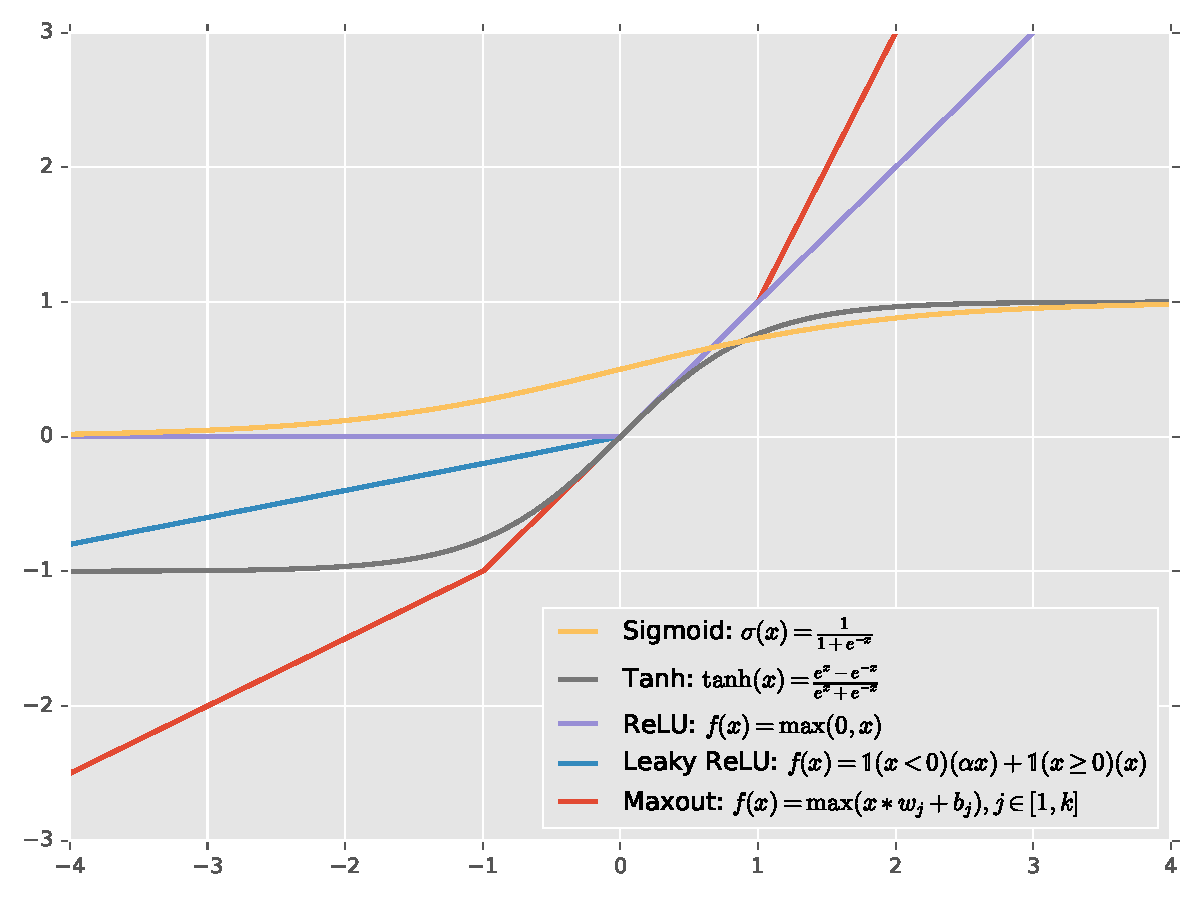
\includegraphics[width=0.6\textwidth]{figure/ch3-activations.pdf}
    \caption{Commonly used activation functions.}
    \label{fig:ch3-activations}
\end{figure}


Depends on the activation, neurons can have different properties and impacts on the whole network. Figure~\ref{fig:ch3-activations} shows most commonly used activation functions:

\begin{description}[labelindent=1cm]
  \item[Sigmoid] Sigmoid is used historically to simulate the firing rate of a neuron but recent years falls out of favor and is rarely used now. It saturates at either tail of 0 or 1, and at these regions the gradient is almost zero, thus it kills gradients from propagating to previous layers, making deep networks not trainable. Another drawback of sigmoid activation is that neurons in later layers will not receive zero-centered inputs, this will cause all positive or negative gradients on the weights during backpropagation, which may lead to undesirable zig-zagging dynamics in the gradient updates of the weights. However, once gradients are added up across a batch of data, the final update for the weights can have variable signs, somewhat mitigating this issue.
  \item[Tanh] Though similar to sigmoid non-linerality in that it also suffers from saturization and thus vanishing gradients problems, tanh is always preferred to sigmoid because its output is zero centered.
  \item[ReLU] Rectified linear unit becomes popular in recent years. \cite{krizhevsky2012imagenet} used it in their winning 2012 ImageNet competetion and found that it greatly accelerated the convergence of stochastic gradient descent optimization process. Also comparing to other activations, it is a much more light weight operation since it is a simple thresholding operation. However, ReLU unit can "die" if a large enough gradient changes the weights such that the neuron never activates on new data.
  \item[Leaky ReLU] Similar to ReLU, but can help fix the "dying ReLU" problem by modifying the flat side of ReLU to have a small gradient~\cite{he2015delving}.
  \item[Maxout] Introduced in~\cite{goodfellow2013maxout}, Maxout unit enjoys all the benefits of a ReLU unit, and does not have its drawbacks. Maxout activation can implement ReLU activtions and approximate any convex activation function.
\end{description}


\subsubsection{Basic Network Structure}
With appropriate loss function, a single hidden unit can function as a linear classifier. However, due to simplicity, its representation power is limited. For example, XOR operation can not be implemented with a single unit, but can be implemented with 3 units. For the network to have enough learning capacity to solve complicate tasks, hidden units are usually aggregated and stacked to form a layer by layer structure. With appropriate regularization, the network can learn powerful features and perform well for many tasks. A regular neural network is shown in Fig~\ref{fig:ch3-ann}, a deep neural network can have many hidden layers. \cite{links:nnplayground} provides an interactive play ground for tinkering with neural networks.


\begin{figure}[t]
    \centering
    \begin{tikzpicture}
        [nodestyle/.style = {circle, inner sep=0pt, minimum size=10pt},
         outstyle/.style = {-latex'new, arrowhead=0.2cm}]

        \foreach \name / \y in {1,...,10}
            \node[nodestyle, fill=black!50] (I-\name) at (0, -\y/2) {};

        \foreach \name / \y in {1,...,12}
            \node[nodestyle, fill=blue!50] (H-\name) at (2, -\y/2 + 0.5) {};

        \foreach \name / \y [count=\i from 0] in {1,...,10}
            \node[nodestyle, fill=red!50] (S-\name) at (4, -\y/2) {\i};

        \draw[dotted, thick, black!50] (I-10) ++(0cm,-0.3cm) -- ++(0cm, -1cm);
        \draw[dotted, thick, blue!50] (H-12) ++(0cm,-0.3cm) -- ++(0cm, -1cm);
        \draw[dotted, thick] (I-10) ++(0cm,-0.3cm) -- ++(0cm, -1cm);

        \foreach \source in {1,...,10}{
            \foreach \dest in {1,...,12}{
                \path (I-\source) edge[outstyle] (H-\dest);
                \path (H-\dest) edge[outstyle] (S-\source);
            }
        \draw[outstyle] (S-\source) -- ++(0.5cm, 0cm);
        }

        \node[text width=8em, text centered, above of=H-1, node distance=0.5cm, font=\tiny] (hl) {Hidden layer};
        \node[text width=8em, text centered, left of=hl, font=\tiny, xshift=-1cm] {Input image};
        \node[text width=8em, text centered, right of=hl, font=\tiny, xshift=1cm] {Output probabilities};

        \node[draw=blue!50, inner sep=0] (mnistres) [below right of=H-12, shift={(4cm,1cm)}] {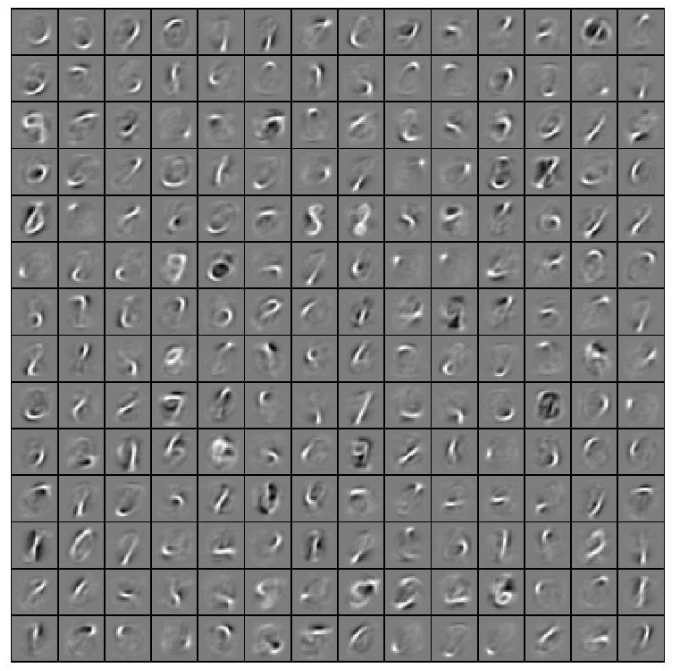
\includegraphics[width=3cm]{figure/dep/mnistresult.png}};
        \node[draw=black!50, inner sep=0] (mnistimg) [left of=I-4, shift={(-0.2cm,0)}] {
\includegraphics[width=1cm]{figure/dep/mnist.png}};
        \node[draw=blue!50, rectangle, inner sep=0, minimum width=0.5cm, minimum height=7.2cm] (fmaps) [above of=H-10, yshift=0.15cm] {};
        % \path (fmaps.north east)  edge [outstyle, bend left, blue!50, out=40] (mnistres.north);
        \node[draw=black!50, rectangle, inner sep=0, minimum width=0.5cm, minimum height=6.1cm] (aimg) [above of=I-9, yshift=0.15cm] {};
        \path (aimg.north west)  edge [outstyle, bend right, black!50] (mnistimg.north);
        \def\rectanglepath{-- +(0.2cm,0cm) -- +(0.2cm,0.2cm) -- +(0cm,0.2cm) -- cycle}
        \draw[blue!50, thick] (5.26, -5.41) \rectanglepath;
        \draw[rotate=45, blue!50, thick] (H-12) ++(-0.05cm, 0.3cm) ellipse (0.3cm and 0.1cm);
        \draw[outstyle, blue!50, decorate,
        decoration={snake,amplitude=.4mm,segment length=2mm,post length=1mm}]
        (H-12) ++(-0.5cm, -0.07cm) to [bend right] 
        node [below, text width=3cm, align=center, midway, font=\tiny]{kernel(feature filter)} (5.26,-5.31) ;

    \end{tikzpicture}

    \caption{A regular feed forward neural network with 1 hidden layer. A 28x28 mnist digit image is flattened and fed into the network, it outputs probabilities of being a certain digit from 0 to 9. The learned kernel for each hidden unit is also shown.}
    \label{fig:ch3-ann}
\end{figure}

\subsubsection{Backpropagation Algorithm}
During the optimization process of loss function, we need to calculate the gradients with respect to all the weights and update them. A naive way is keep all the weights fixed and only tweak one weight to see how it changes loss, thus get its gradient. However, this method is very inefficient since it has to tweak order of the number of weights times to get gradients for all the weights. The efficient way to do this is backpropagation algorithm. Detailed derivations on backpropagation algorithm can be found on tutorials~\cite{links:nielsennnbook, links:cs231n}. We highlight some points here:
\begin{itemize}
\item It helps to think of the mapping from input to output that the neural network represents as a computational graph. Each node in this computational graph is simple operation like $+$, $*$, $\max$, or any operation like $\sigma$ that have a simple derivable gradients. In such way, any complicate mapping function is decomposed into simple unit operations, and backpropagation refers to the node by node backward propagation of gradients from loss to input using chain rule.
\item There can be many paths from loss to any variable in the network, gradients flowed through all these paths backwards to this variable get added up when calculating gradient on this variable.
\item In neural networks, the preactivations of a layer $z$ and activations of previous layer $o$ have relation $z = w^To$ where $w$ are the weights between these two layers, it can be seen that gradients for $w$ are proportional to activations $o$ of previous layer, this implies that the scale of the data has an effect on the magnitude of gradients for the weights. When input data is not scaled well, the gradient can be huge, so data preprocessing is a good practice.
\end{itemize}

\subsubsection{Training}
Below we list most of the practical concerns when training neural networks:
\begin{description}[labelindent=1cm]
  \item[Data Preprocessing] Common data preprocessing steps include mean subtraction, normalization, PCA whitening~\cite{links:ufldlpca}. Mean subtraction is to zero-center the data. Normalization refers to normalizing the data dimensions so that they are of approximately the same scale. PCA whitening is to first apply PCA on the dataset, followed by a normalization step on the principle components. For most computer vision tasks with big image datasets as input, mean subtraction is enough.
  \item[Weight Initialization] Mostly used weight initialization strategy is random sampling from a damped gaussian distribution. Improvements on randomly initialization are focused on calibrating the variances with respect to number of inputs for each neuron such that its output's variable does not blow up. For ReLU units, it is recommended to draw weights from $\sqrt{\frac{2.0}{n}}\mathcal{N}(0,1)$ as suggested in~\cite{he2015delving}. A recently developed technique called batch normalization explicitly forces each neuron's activations for a minibatch to take on a unit gaussian distribution through whitening among this minibatch~\cite{ioffe2015batch}. Batch normalization can be interpreted as doing preprocessing at every layer of the network, but integrated into the network itself in a differentiable manner. In practice networks that use batch normalization are significantly more robust to bad initialization.
  \item[Regularization] $\mathcal{L}2$ regularization $\frac{1}{2}\lambda w^2$ is still the most commonly used regularization term. Other than that, $\mathcal{L}1$ regularization $\lambda |w|$ leads to sparsity in weights, it is useful when the problem is concerned with explicit feature selection. Dropout~\cite{srivastava2014dropout} is a simple but effective way of regularization, in practice it smears activations with a certain probability during training, which can be interpreted as sampling a neural network within the full neural network, and only updating the parameters of the sampled network based on the input data, therefore effectively there are many more neural nets working as an ensemble to eventually perform the classification.
  \item[Loss Functions] In classification problems, most commonly used data loss functions are hinge loss and cross-entropy loss. Hinge loss is defined as $L_i = \sum_ {j\neq y_i} \max(0, f_j-f_{y_i}+1)$ where $L_i$ and $y_i$ refer to loss and ground truth label of $i$th sample, $f_j$ is the output score for class $j$. Hinge loss is used with SVM classifier. Cross-entropy loss is defined as $L_i = -\log(\frac{e^{f_{y_i}}}{\sum_je^{f_j}})$, and used with Softmax classifier. For regression problems, $\mathcal{L}2$ distance $L_i = ||f - y_i||_2^2$ are normally used. Whenever possible, it is recommended to see if a regression problem can be morphed to a classification problem by quantization of outputs into bins, because classification is an easier task and gives confidences of each class.
  \item[Optimization] There are many optimization options when training deep neural networks. Starting from vanilla SGD (stochastic gradient descent), integration of momentum improves convergence rate and adaptive algorithms ease the pain of tuning the learning rates. \cite{links:sgdoptimization}~gives a comprehensive overview of related algorithms.
  \item[Miscellous] To find good hyperparameters such as initial learning rate, regularization strength, it is suggested to use random search over grid search~\cite{bergstra2012random} and stage the search from coarse to fine. Bagging of neural networks trained independently is a reliable approach to improve the performance.
\end{description}


\section{Convolutional Neural Networks}

\subsection{Architecture Overview}

\subsection{Layers}

\section{Applications}

\subsection{Classification}

\subsection{Detection}


\newpage

% \chapter{Cardea}\label{sec-cardea}

\section{System Design}
Recalling related works in Chapter 2, what motivates the design of Cardea are the follow:

\begin{itemize}
\item People's privacy concerns are dependent on context. Although in certain circumstances locations are strong hints of possible privacy intrusion, generally what individuals are doing and with whom are more essential and crucial factors that directly relate to privacy.
\item People's privacy preferences vary from each other, thus they should be able to express their personal privacy preferences.
\item People's privacy preferences may change from time to time, therefore they need a way to change such preferences easily.
\end{itemize}

To achieve these objectives, we propose following solution:
\begin{itemize}
  \item We combine GPS location, grouped scene categories (Table~\ref{tbl-scenecate}) and accompanied persons as context that can better represent people's privacy concerns than previous methods. As a result we are able to provide more general as well as finer granularity privacy preference settings for users.
\item We use cloud server to host individualized privacy preferences, and user's preference is binded with his facial features. In this way his raw visual information stays locally, preventing the case of visual privacy leakage from hacked servers.
\item Other than a simple interface provided to users to update their privacy preferences, hand gestures like \vcenteredinclude{figure/ch4-yesgesticon.png} and \vcenteredinclude{figure/ch4-nogesticon.png} can be used by user to actively speak out about his preference in the capturing moment, enriching the interaction and adding more flexibilities.
\end{itemize}
As introduced in chapter 3, breakthroughs made by deep learning community in many computer vision problems such as image classification, face recognition and object detection have guided the proposed solution and shed lights on its practicability. More specifically, given a captured image, Cardea will leverage powerful convolutional neural networks to for the recognition of scene context, registered users and gestures. Cardea's design is given in Fig~\ref{fig:ch4-cardeadesign}, it is composed of the client applications and cloud server. It works based on data exchange and collaborative computing involving both client and cloud sides. The major components and interactions include:
\begin{figure}[!htbp]
    \centering
    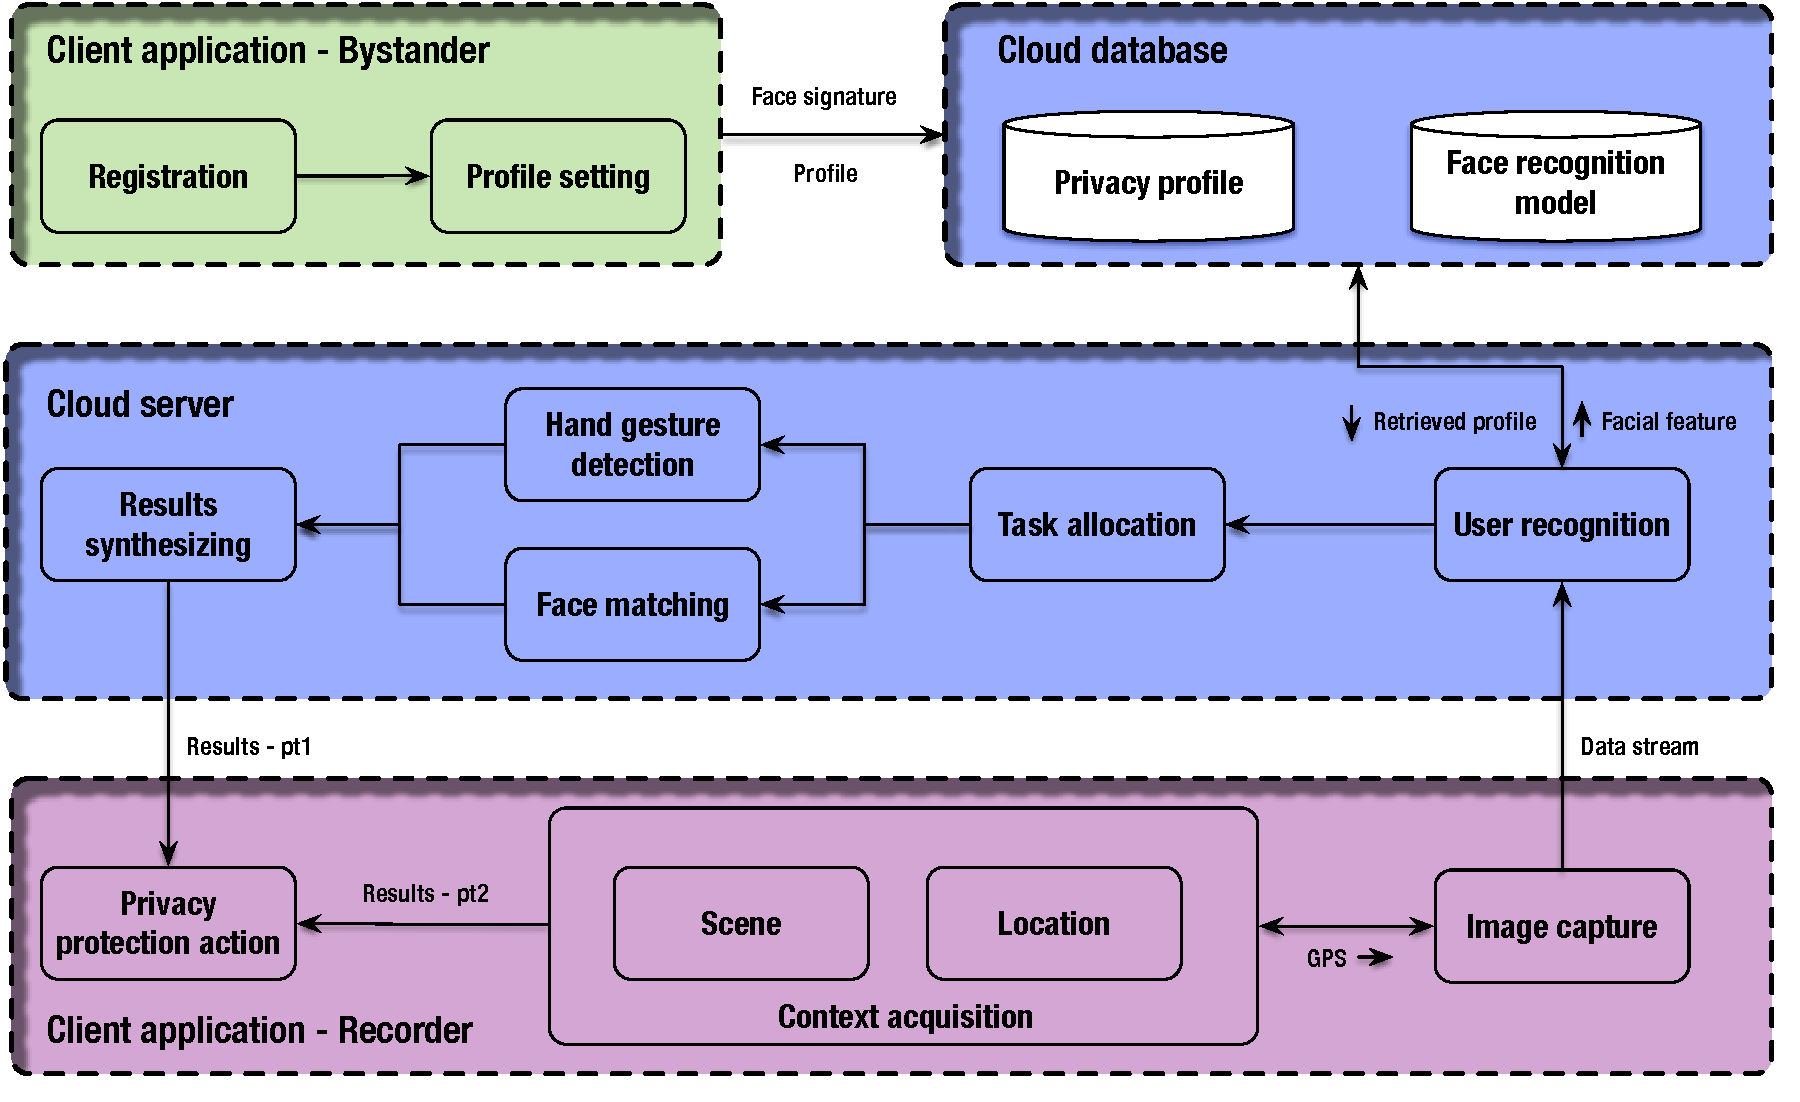
\includegraphics[width=1.0\textwidth]{figure/ch4-cardeadesign.pdf}
    \caption{System design of Cardea.}
    \label{fig:ch4-cardeadesign}
\end{figure}

\begin{description}[leftmargin=0cm]
  \item[{\bfseries Bystander client application:}] A bystander can use this application to register as Cardea user and define his privacy profile. It will capture a number of face images (about 50–60 images) and extract facial features from these images as his unique face signature. After setting up the context dependant privacy preference, his facial signature and preference will be sent to cloud server for registration and updating of face recognition model.
  \item[{\bfseries Recorder client application:}] A recorder can use this application to take images that will automatically perform privacy protection actions in compliance with all Cardea users' privacy preferences. Given a captured image, it first detects all the faces and extracts the corresponding facial features locally on device, then the features and the captured image but is compressed and with all detected faces blurred are sent to the server for face and gesture recognitions. GPS coordinate is also sent to server in this step to be compared with recognized users' location settings. During the time waiting for response from cloud, it performs scene group prediction task. Finally, predicted scene group and intermediate decision result received from server are used to decide the actual protection action which will be enforced on the raw captured image.
  \item[{\bfseries Cloud server:}] The cloud server serves as two roles: \ding{182} When receives requests from Bystander applications, it will store/update users' profiles, and training/updating system's face recognition model automatically; \ding{183} When receive requests from Recorder applications, it will initiate face and gesture recognition tasks, as well as partial decision making based on recognition results, and send these intermediate decision results to client for final step of decision making.
\end{description}

% Implementations of each module, how Cardea allocates tasks between mobile and cloud, integration, usage and performance evaluation of the whole system are discussed throughly in following sections.

Implementations and evaluation of each module, how Cardea allocates tasks between mobile and cloud, integration and user interactions are discussed in following sections.

\begin{table}[tb]
\centering
\caption{Scene categories.}
\label{tbl-scenecate}
\begin{tabular}{ll}
\toprule
Scene Group    & Scene Category                                       \\ \midrule
Eating         & bistro/indoor, bistro/outdoor, cafeteria, coffee\_shop, \\
               & diner/outdoor, dining\_hall, dining\_room, fastfood\_restaurant, food\_court, \\
               & restaurant, restaurant\_patio, sushi\_bar            \\ \midrule
Entertainment  & bar, discotheque, pub/indoor                         \\ \midrule
Shopping       & bazaar/indoor, bazaar/outdoor, clothing\_store, general\_store/indoor, \\
               & jewelry\_shop, shoe\_shop, shopping\_mall/indoor, supermarket  \\ \midrule
Work           & conference\_center, conference\_room, cubicle/office, library/indoor, office, \\
               & office\_cubicles, reading\_room                      \\ \midrule
Public         & park, street                                         \\ \midrule
Mobility       & airplane\_cabin, airport\_terminal, bus\_interior, bus\_station/indoor, \\
               & subway\_station/platform, train\_interior, train\_station/platform \\ \midrule
Exhibition     & art\_gallery, museum/indoor                          \\ \midrule
Religion       & cathedral/indoor, cathedral/outdoor, church/indoor, church/outdoor, mosque/outdoor, \\
               & pulpit, temple/east\_asia, temple/south\_asia        \\ \midrule
Illness        & hospital, hospital\_room, nursing\_home                \\ \midrule
Nudity         & bathroom, beach, jacuzzi/indoor, sauna, shower, \\
               & swimming\_pool/indoor, swimming\_pool/outdoor        \\ \bottomrule
\end{tabular}
\end{table}

\section{Model Training}

\subsection{Scene Classification}

\subsubsection{Data Preparing and Preprocessing}

For scene classification, we use pre-trained model of Places2 dataset provided by~\cite{links:places2mit}. In the time Cardea project was conducted, Places2 dataset provided by the authors contained 401 categories with more than 8 million training images, and the pre-trained model was based on AlexNet structure~\cite{krizhevsky2012imagenet}. By the time this thesis is writing, the dataset is deprecated and the new Places2 dataset contains 365 categories. And the authors provide more pre-trained models based on different network structures~\cite{links:places2pre}.

\begin{figure}[!htbp]
    \centering
    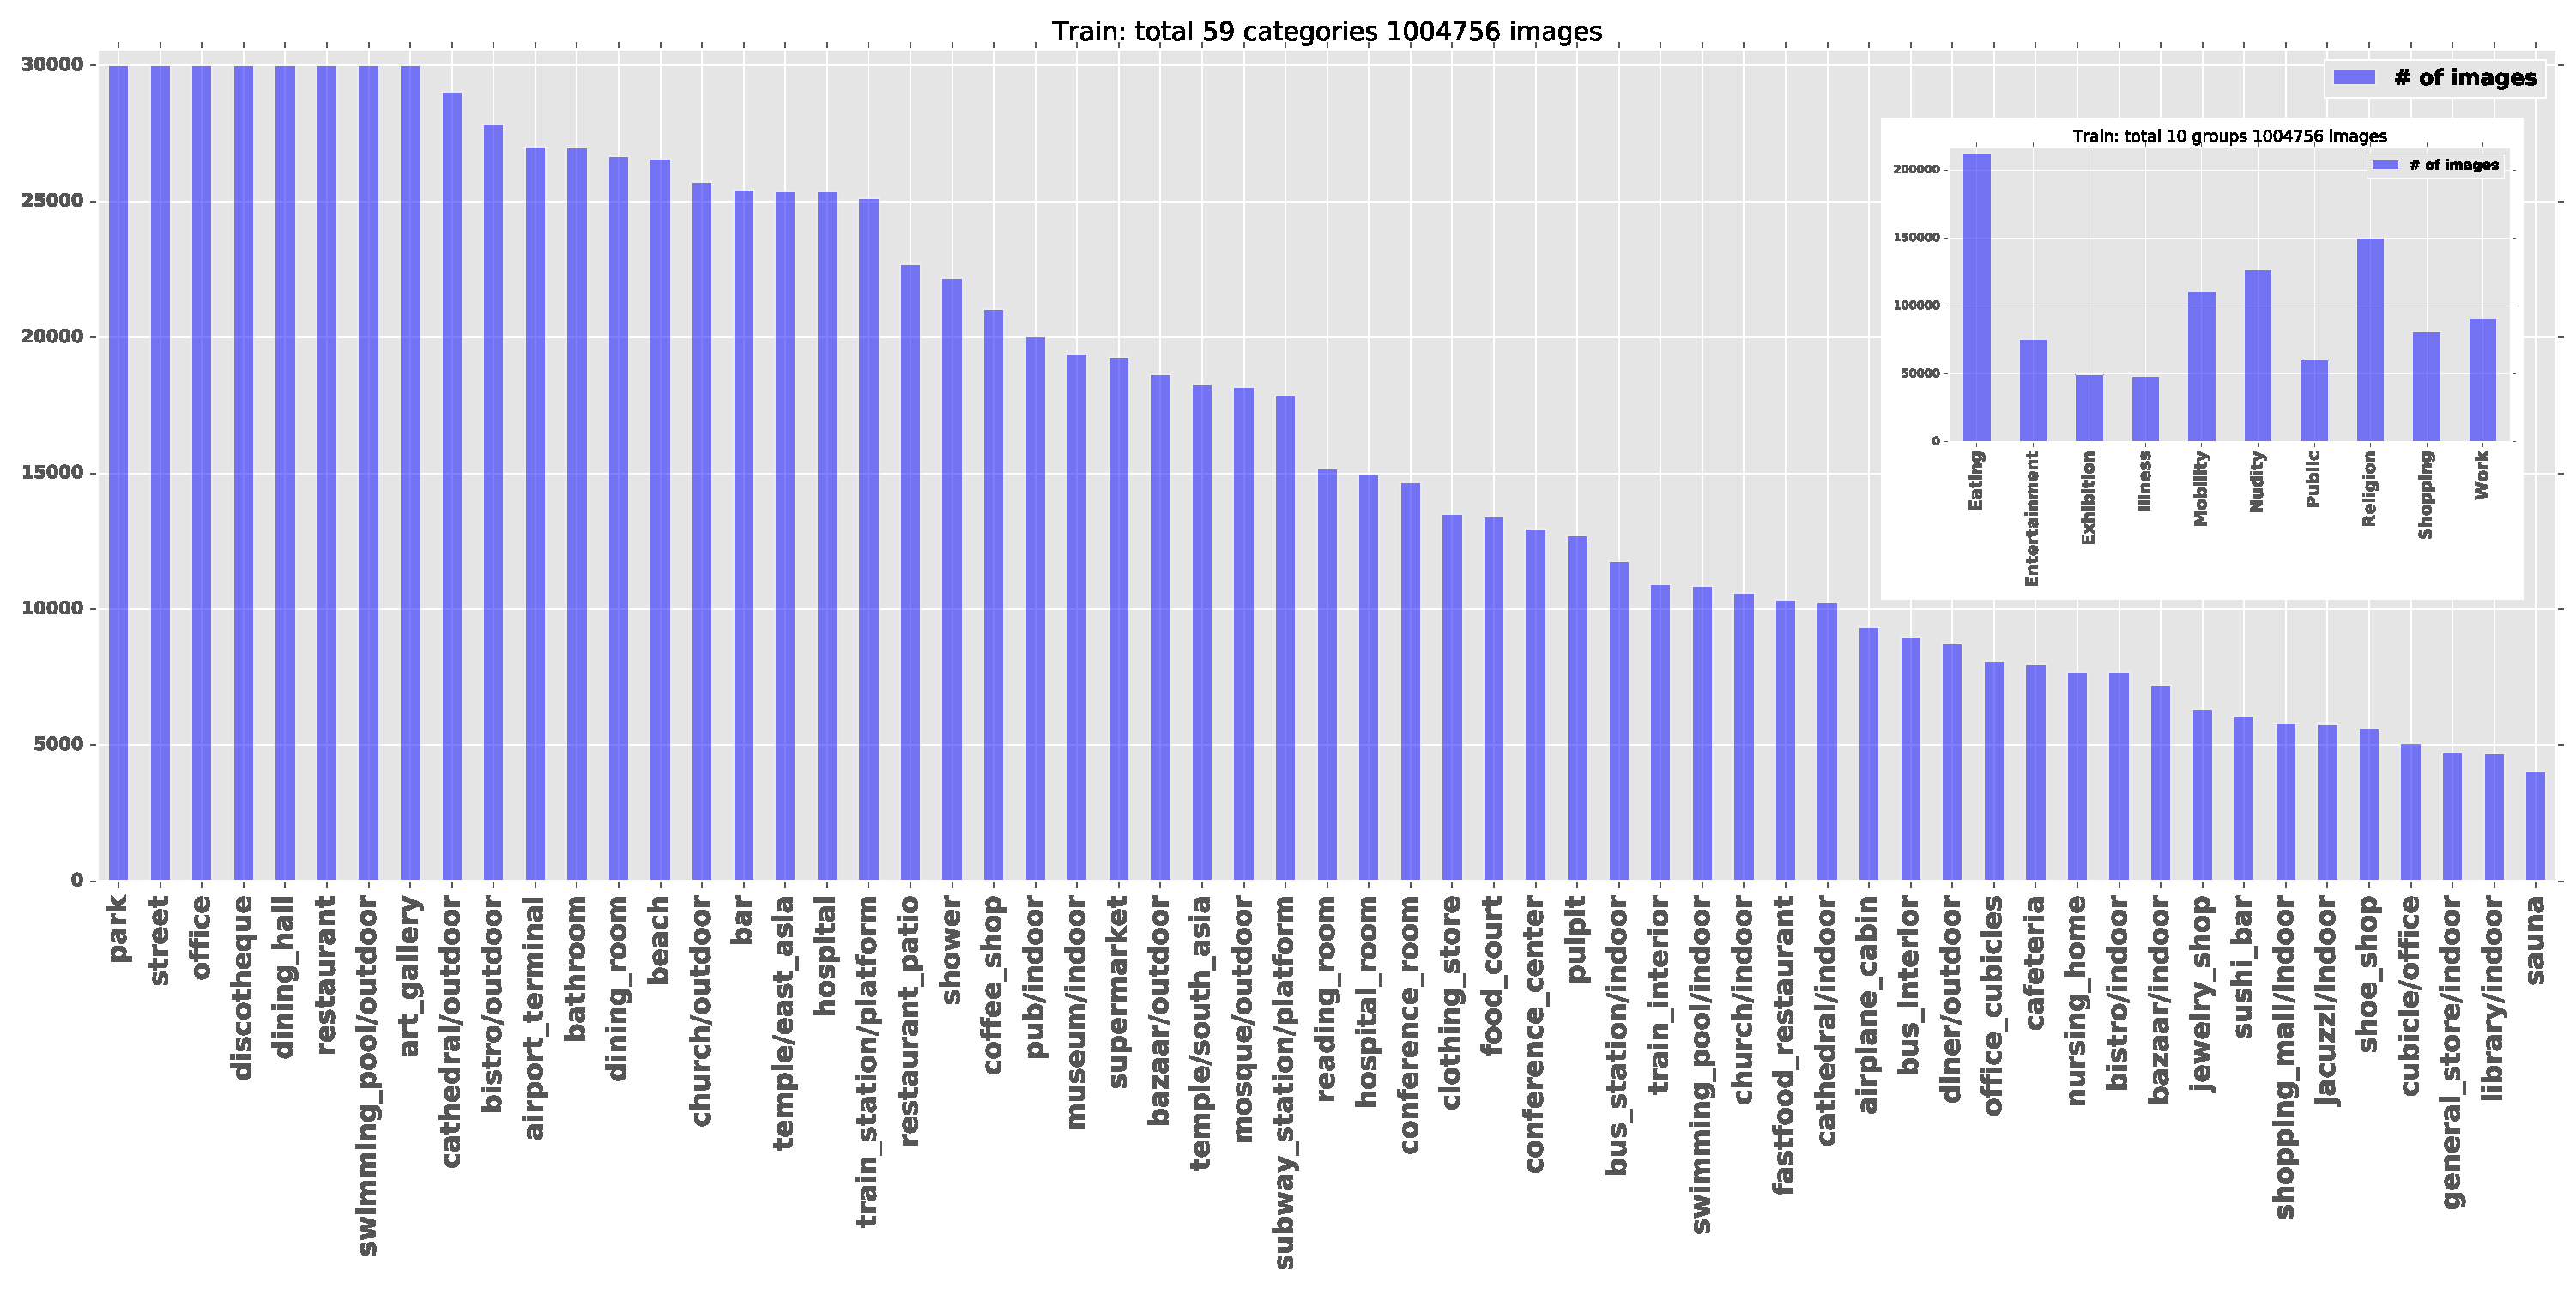
\includegraphics[width=1.0\textwidth]{figure/ch4-numdist.pdf}
    \caption{Number of images for each category and each group (inset).}
    \label{fig:ch4-scenenumdist}
\end{figure}

Note that in the dataset we used, there is a non-uniform distribution of images per category for training, ranging from 4,000 to 30,000, mimicking a more natural frequency of occurrence of the scene. Among the 401 categories, we choose 59 scene categories that are close to daily life and in such scenes people may have privacy concern. In total this subset composed of 1 million training images and 2950 validation images (50 validation images for each category). We also group these 59 scene categories into 10 groups based on contextual similarity as shown in Table~\ref{tbl-scenecate}, such that people have similar reasons for privacy in scenes that are in the same group (e.g. people don't want to be captured in bathroom and beach is both because of nudity concerns). The distribution of training images among categories and groups is shown in Fig~\ref{fig:ch4-scenenumdist}.

\subsubsection{Training Procedures}
Our training step is just a standard fine-tuning process, which is extensively used in transfer learning~\cite{sharif2014cnn,yosinski2014transferable}:

\begin{itemize}
\item[\ding{182}] Using pre-trained model as feature extractor, we extract the features at \emph{fc7} layer for images belonging to the 59 picked categories. Other than shuffling the features, we also augment the features such that all categories have same amount of features. Though the natural frequencies of occurrence are obviously different among different scenes, we argue that for the purpose of privacy protection, all the scene categories should be equally important, thus categories imbalance is not what we favored. The augmentation step can be implemented using weighted loss layer, but we take simple way of bootstrapping features for categories with less images. After this step, all features are cached and stored in lmdb format.
\item[\ding{183}] Train a softmax classifier of the 59 categories using the extracted features. We choose to train a classifier for categories and then add up the output probabilities to predict the group, rather than directly train a group classifier, is because category classifier tells more about the image, and our desired property is equal weights among scene categories rather than groups.
\item[\ding{184}] Both feature extraction and classifier training are implemented using Caffe library~\cite{links:caffelib,jia2014caffe}. In this step we merge the feature extraction part of pre-trained model and the softmax classifier into a single model by copying weights. Now Caffe has the option of specifying layers with fixed weights, thus simplifying the fine-tuning and deployment process.
\end{itemize}

Other than improving the validation accuracy from 0.56 to 0.57, shuffling also makes training converges faster. With augmentation to relieve category imbalance issue, the classifier can finally achieve 0.600 validation accuracy on the 59 categories. There is no other benchmarking result specifically on the subset we choose, but recent benchmark gives 53\%-56\% validation accuracy on the new Places2 dataset with 365 categories~\cite{links:places2pre}, suggesting our model is competitive. The higher validation accuracy of our model is due to the smaller scale of classification problem we are dealing with.

\subsubsection{Prediction}

\begin{figure}[!t]
    \centering
    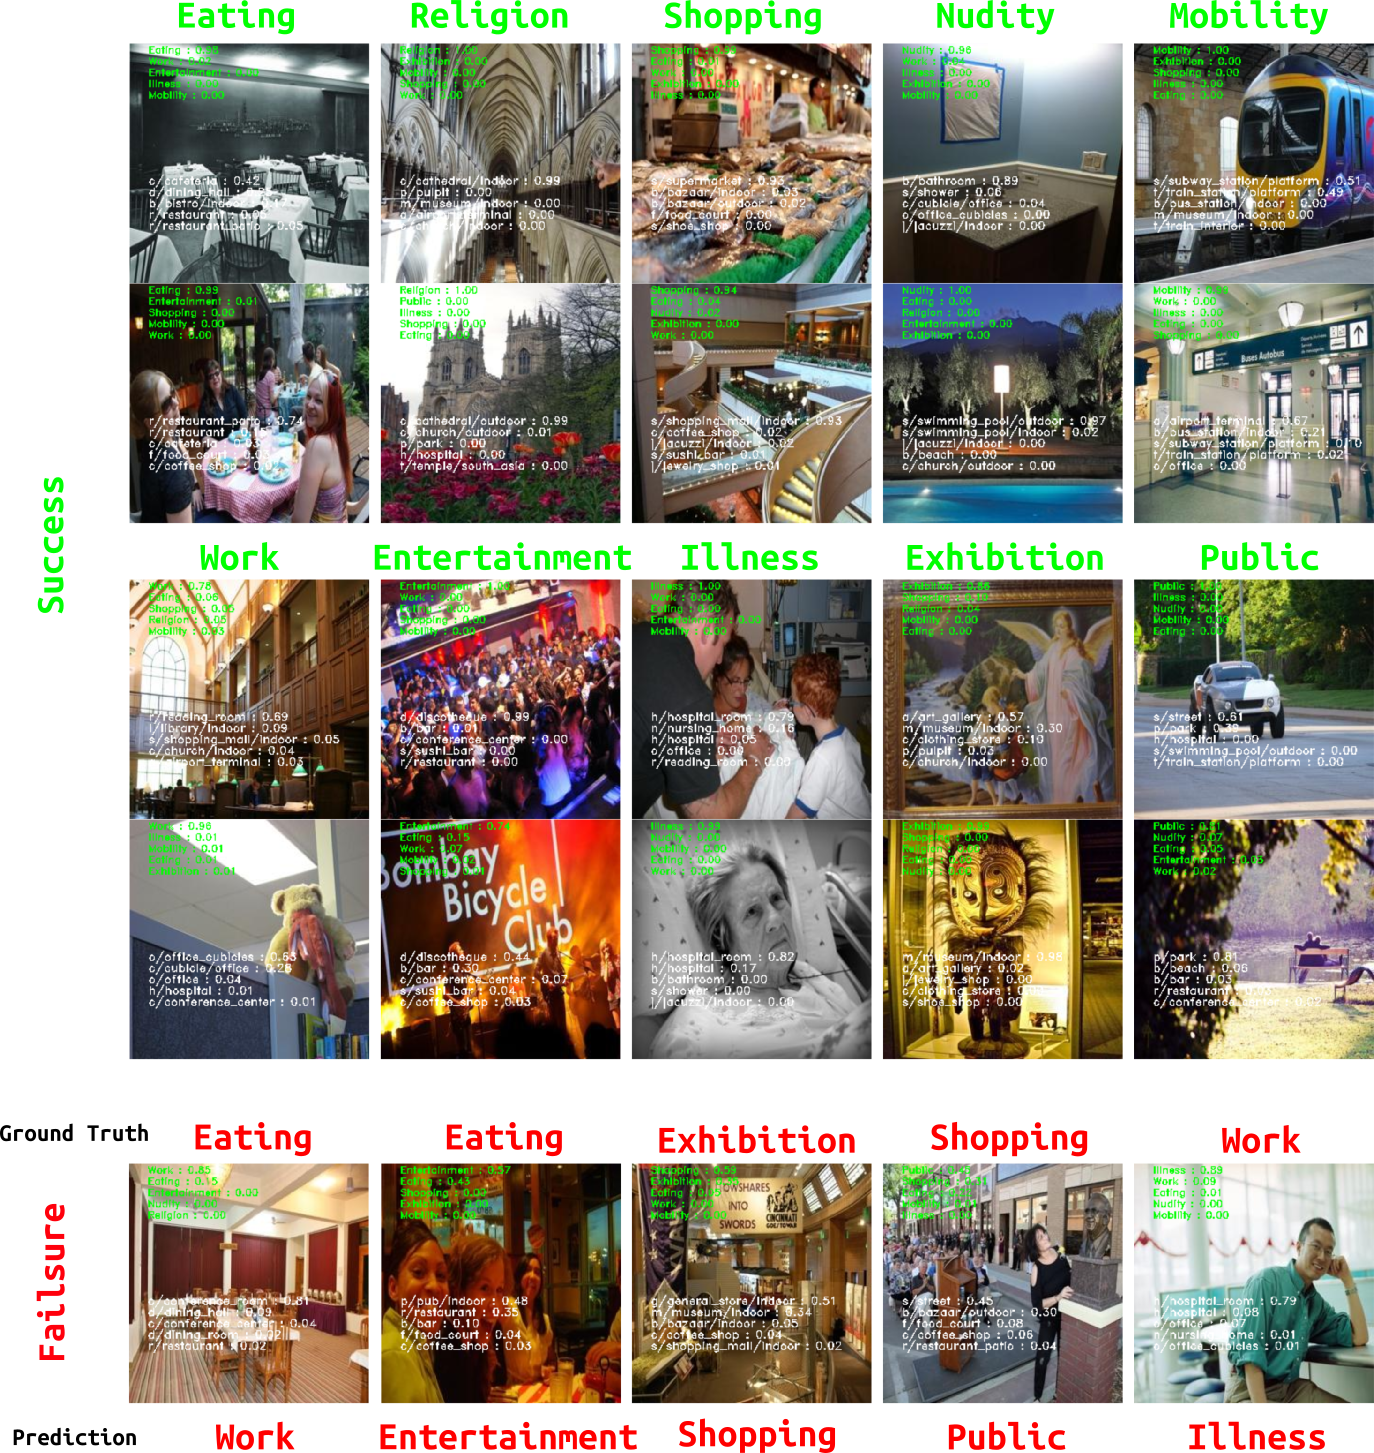
\includegraphics[width=\textwidth]{figure/ch4-scnpredictemp.png}
    \caption{Scene classification prediction example. Top5 groups (green) and categories (white) are shown with their probabilities.}
    \label{fig:ch4-scnpredictemp}
\end{figure}

For prediction, we get probability of a group by summing up the probabilities of all categories belonging to this group, and output the most probable group as prediction of an image. Our model's group prediction accuracy for the validation set is 82.8\%. Fig~\ref{fig:ch4-scnpredictemp} shows some prediction examples. As seen from the examples, given an image, the predicted category probabilities are usually distributed to few categories within same group, thus group prediction is resilient to perturbation of category prediction. The way we group categories can be seemed as a hard-coded clustering step, which makes prediction more robust to noise. The failure cases are mostly due to natural context ambiguity from a image (e.g. image with object in focus, therefore not enough hints for scene inference). Labeling the 342 non selected categories as extra group will amplify the ambiguity issue, even for images with less ambiguity, doing so will distribute probabilities to the extra group and lead to wrong prediction. In other words, a 59 way classifier leads to higher recall for selected scenes and grouping leads to higher accuracy. This is also reflected in confusion matrices shown in Fig~\ref{fig:ch4-scnconfumat}, category confusion matrix shows some clustering structure which is in accordance with the groups we manually assigned. However, only using top 1 category for prediction sacrifices prediction accuracy, which can be avoided by grouping as shown in group confusion matrix.

\begin{figure}[!htbp]
    \makebox[\textwidth]{
        \centering
        \raisebox{-0.5\height}{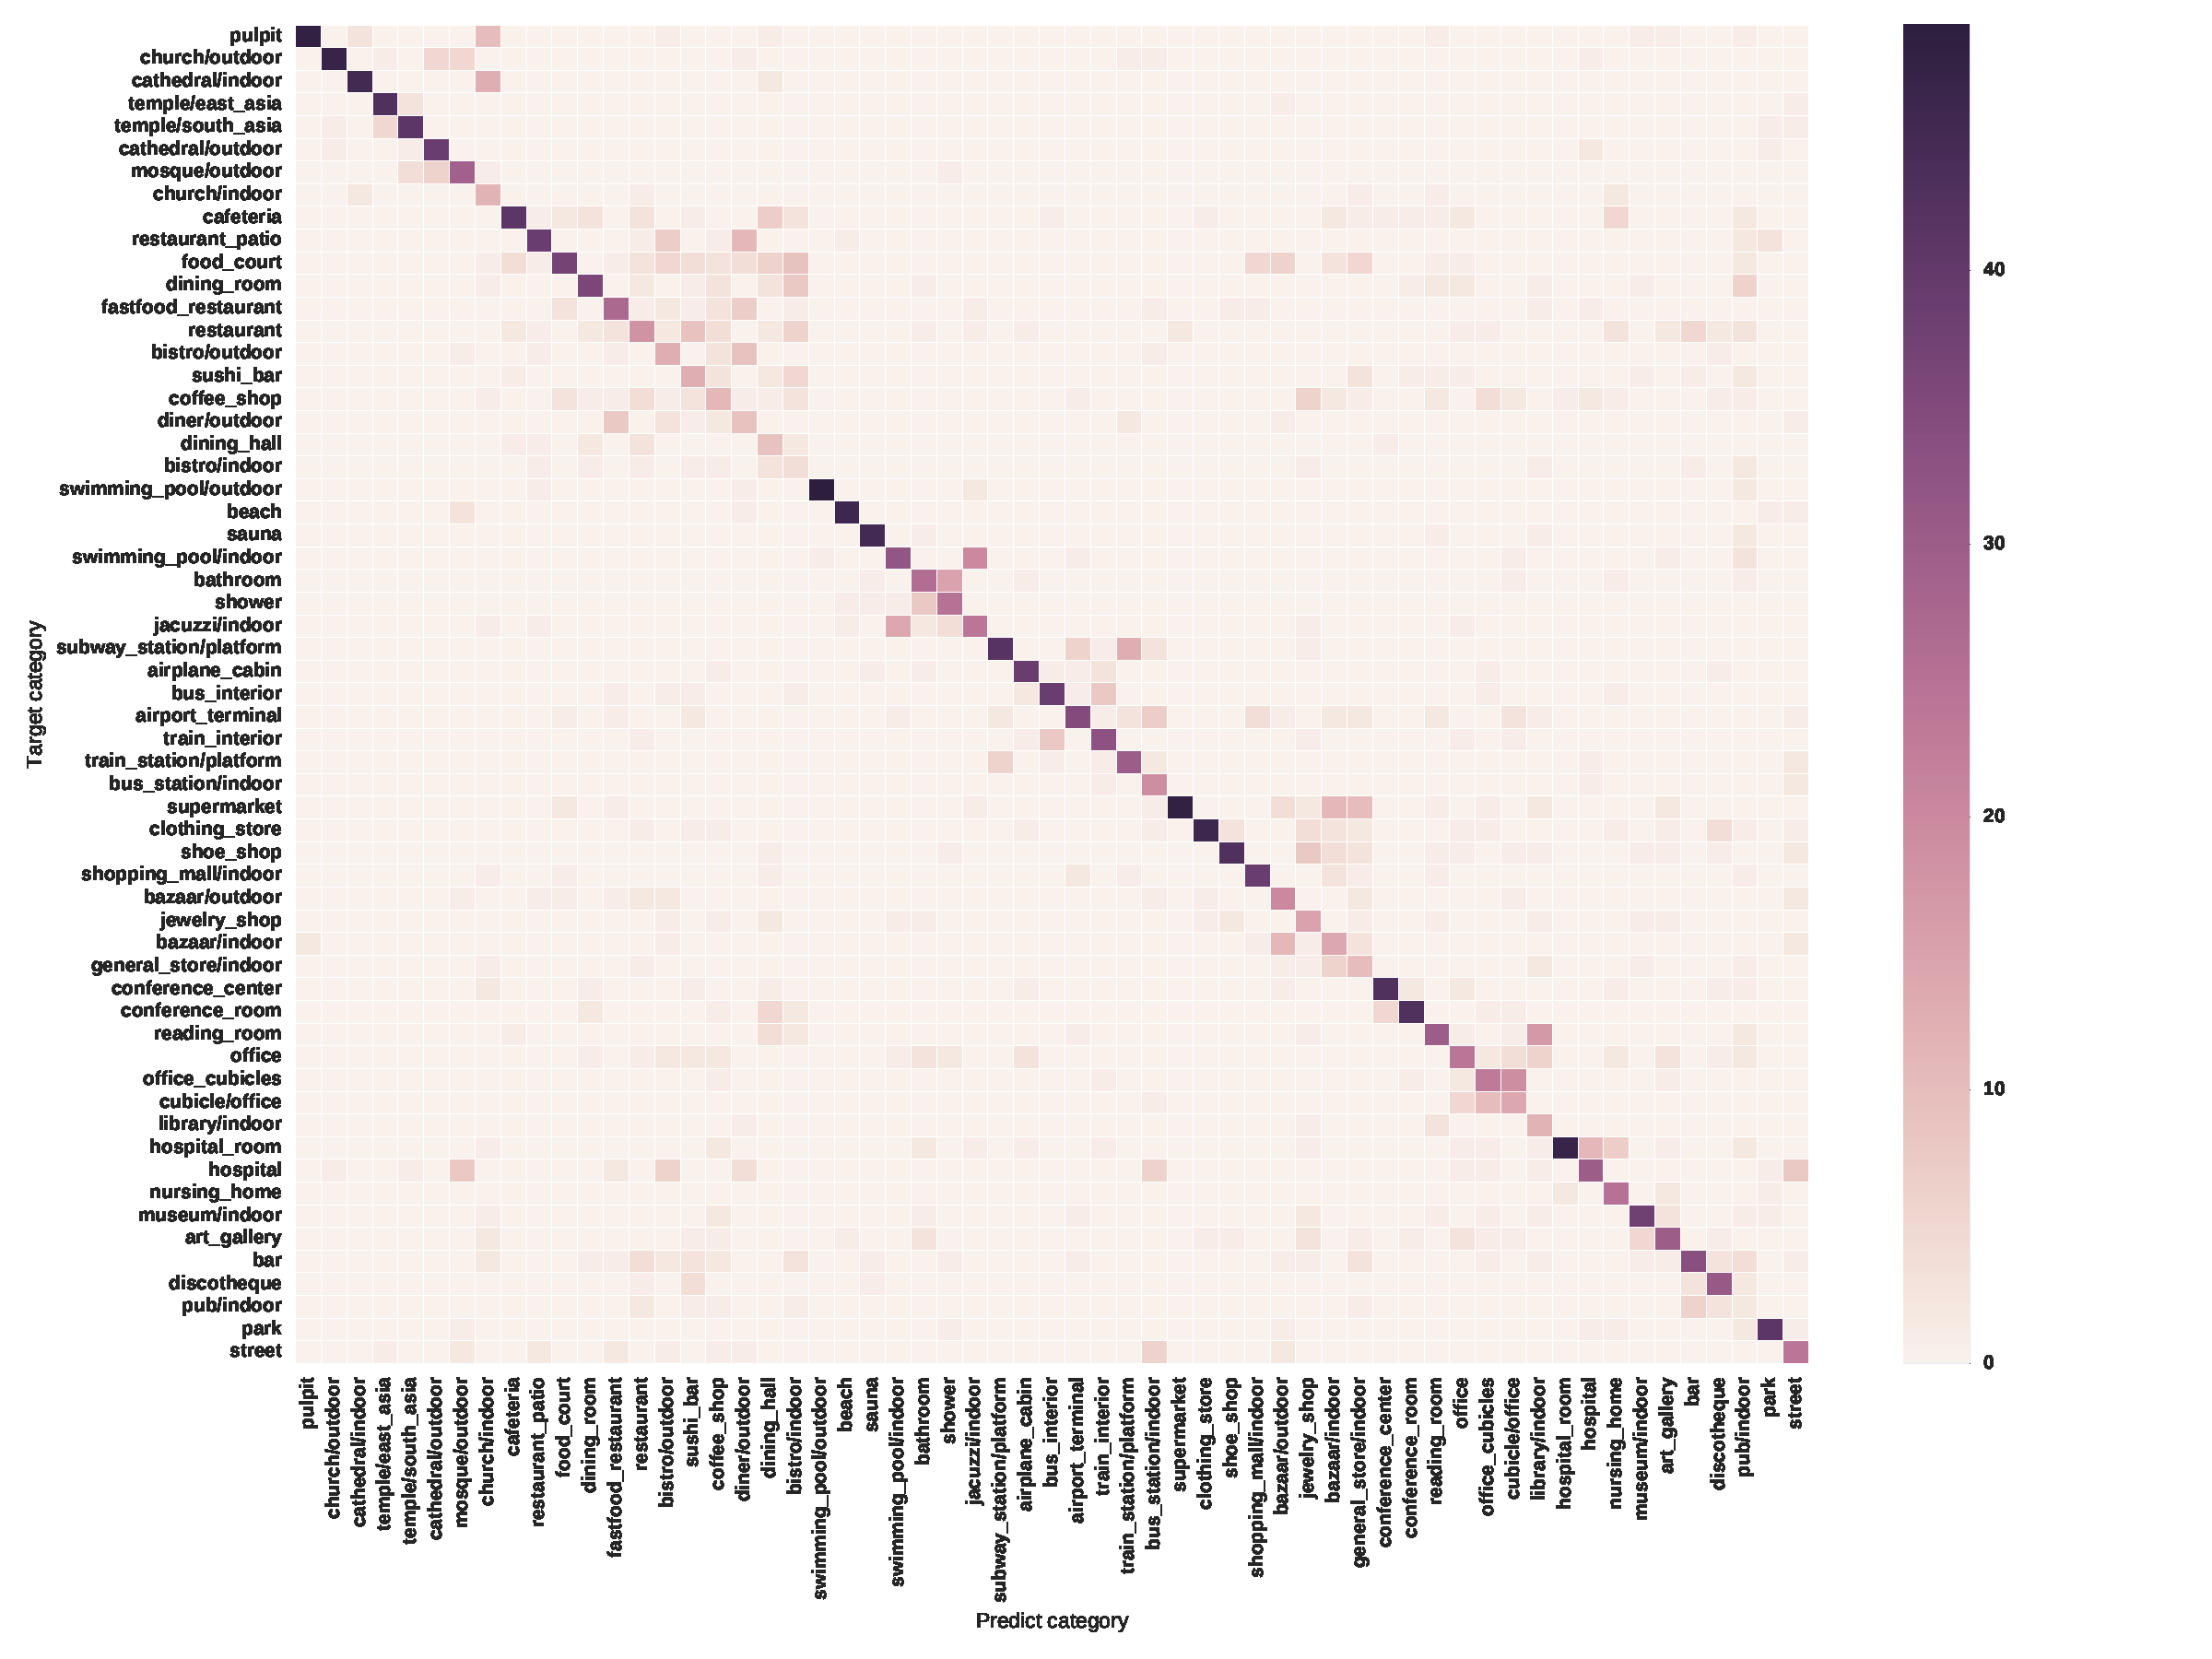
\includegraphics[width=0.7\textwidth]{figure/ch4-scnCateConfu.pdf}}
        \hspace{-1cm}%
        \raisebox{-0.5\height}{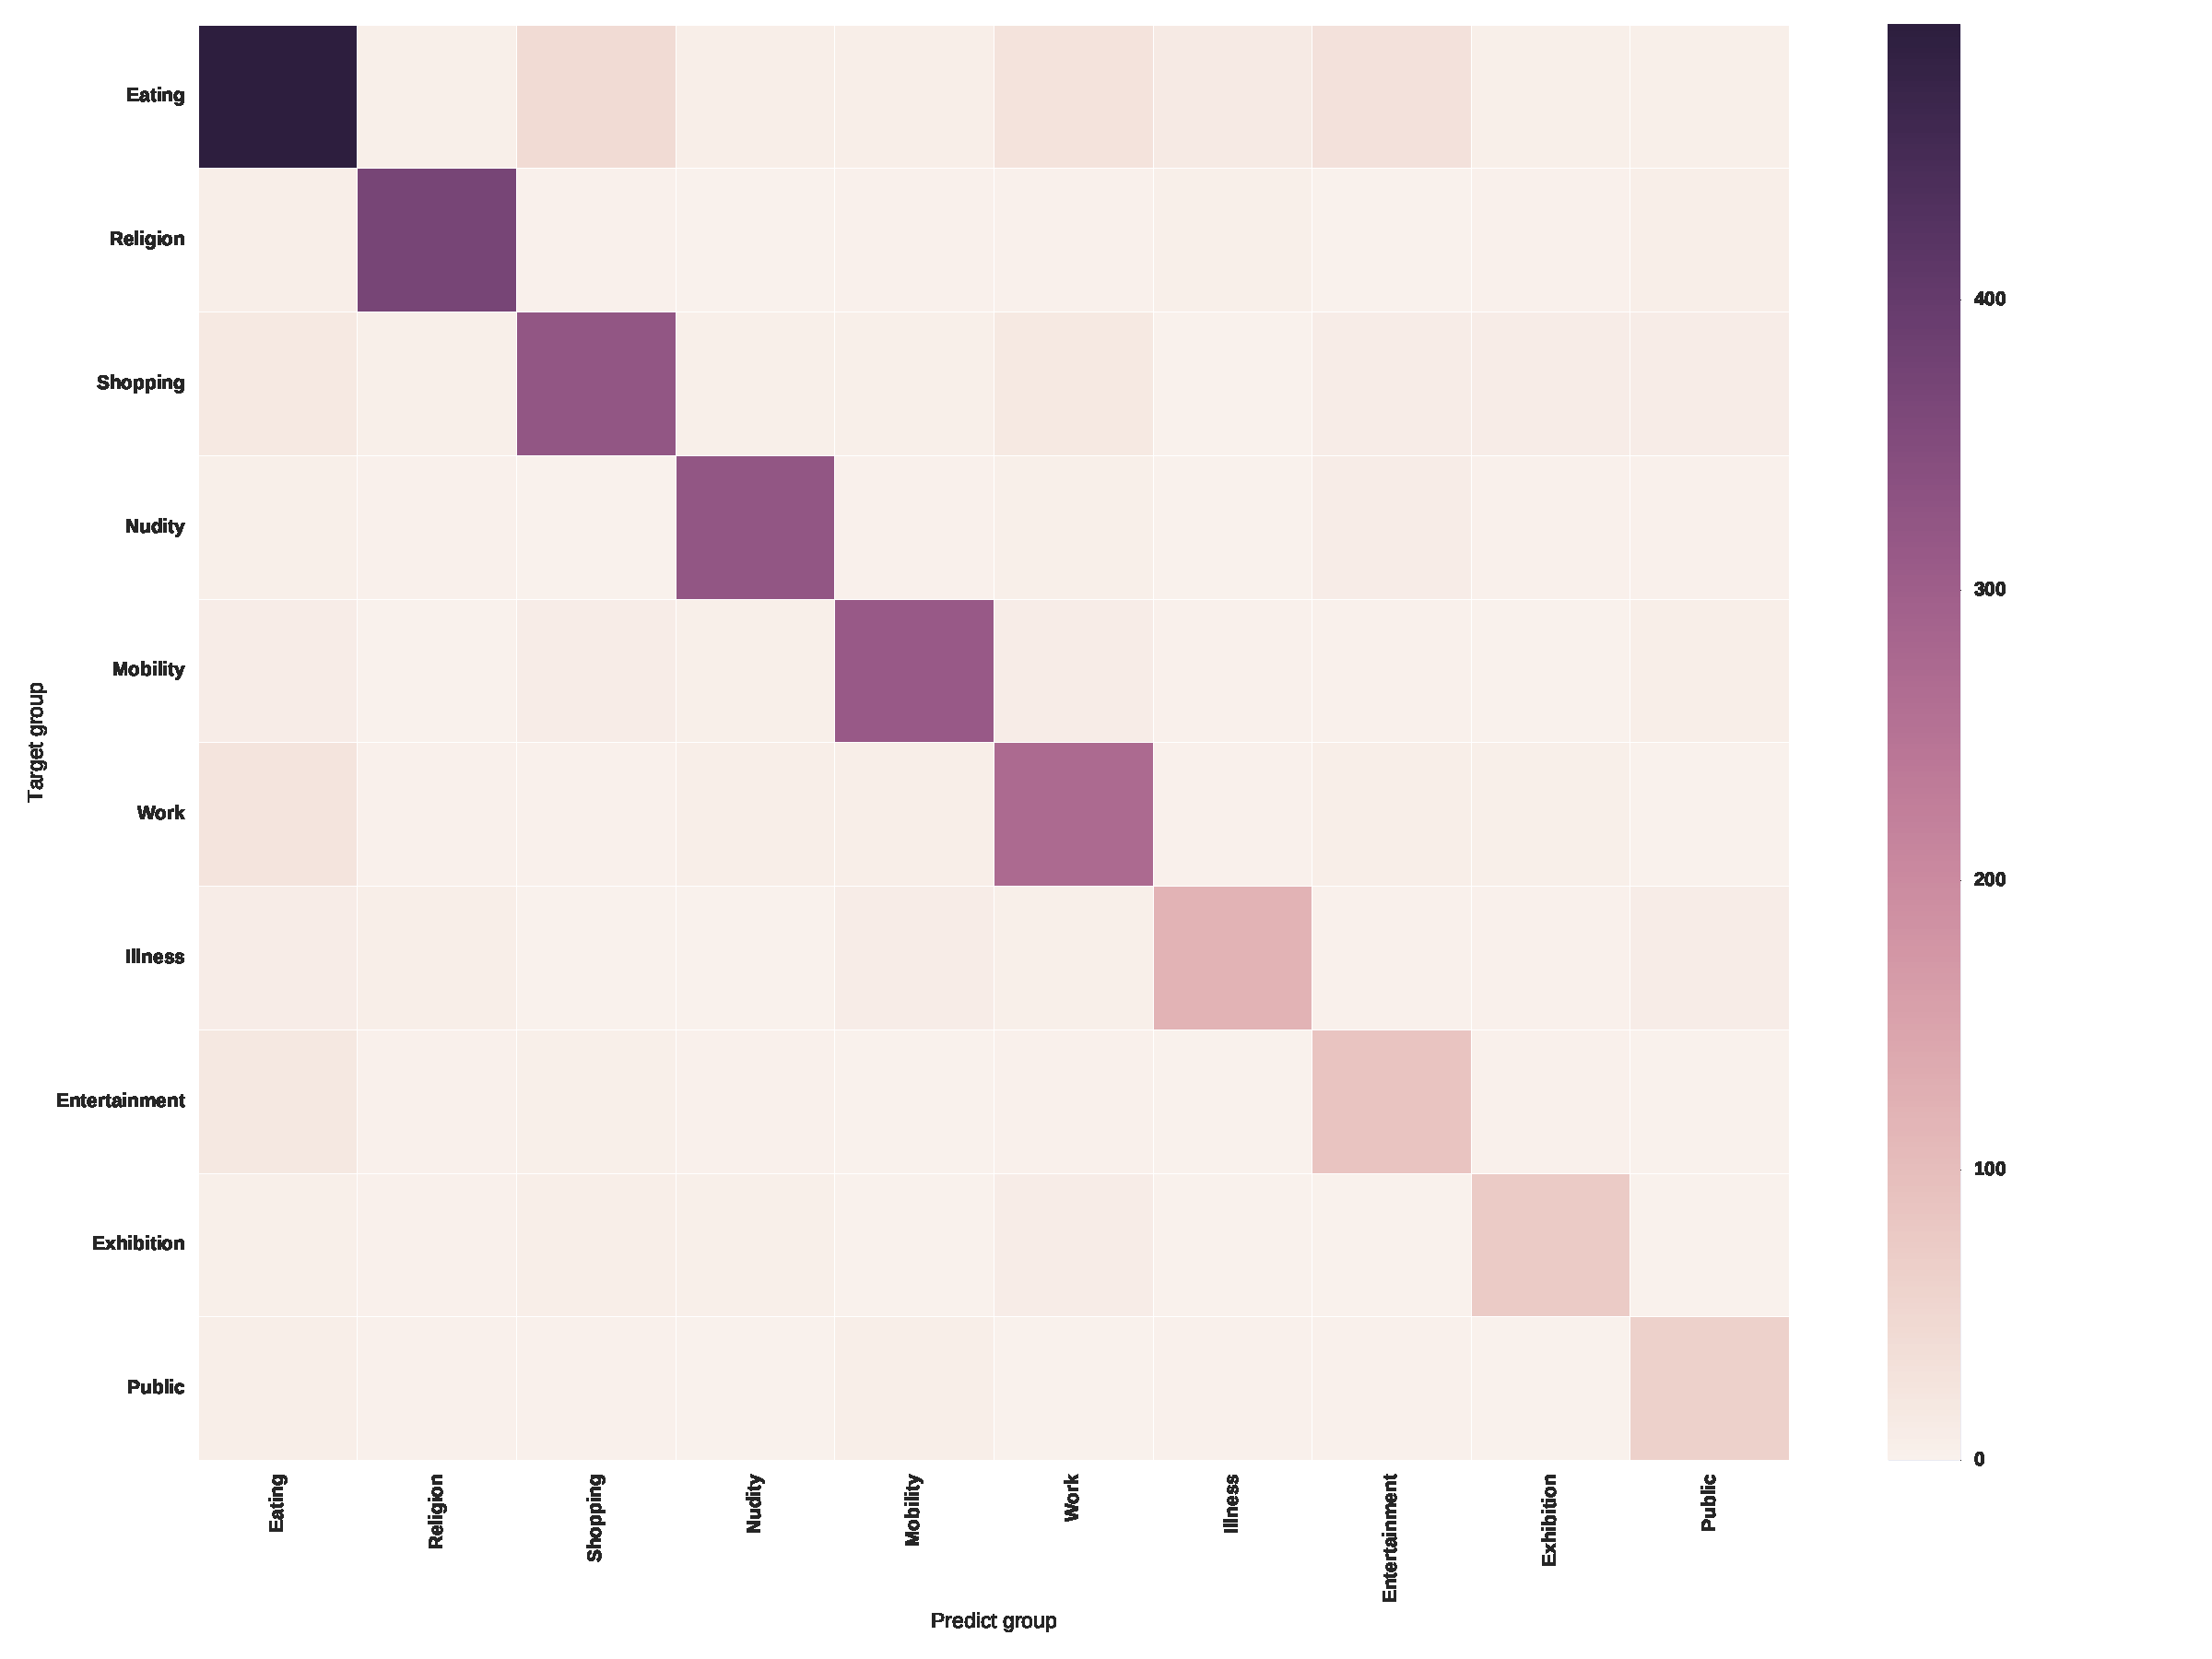
\includegraphics[width=0.6\textwidth]{figure/ch4-scnGrpConfu.pdf}}
    }
    \caption{Confusion matrices for category prediction (left) and group prediction (right).}
    \label{fig:ch4-scnconfumat}
\end{figure}



\subsection{Face Recognition}
Like scene classification, we select a pre-trained model for face recognition task. More specifically, the pre-trained model will serve as face feature extractor, and we will update the face classifier whenever new users register in Cardea and upload their face features. There are already many deep neural networks deployed in commercial products, like Megvii's Face++~\cite{zhou2013extensive}, Facebook's Deepface~\cite{taigman2014deepface}, Google's Facenet~\cite{schroff2015facenet}, Sensetime's Deepid~\cite{sun2015deepid3}. OpenFace~\cite{amos2016openface} is an open source project that is gaining attentions in recent months, it is based on Torch~\cite{links:torch7}. Because Cardea's other modules are under Caffe framework, we limit our options on open sourced Caffe models. The models in our consideration are VGG face recognition model~\cite{parkhi2015deep} and Lightened CNN face recognition model~\cite{wu2015lightened}.

\begin{figure}[!htbp]
    \makebox[\textwidth]{
        \centering
        \raisebox{-0.5\height}{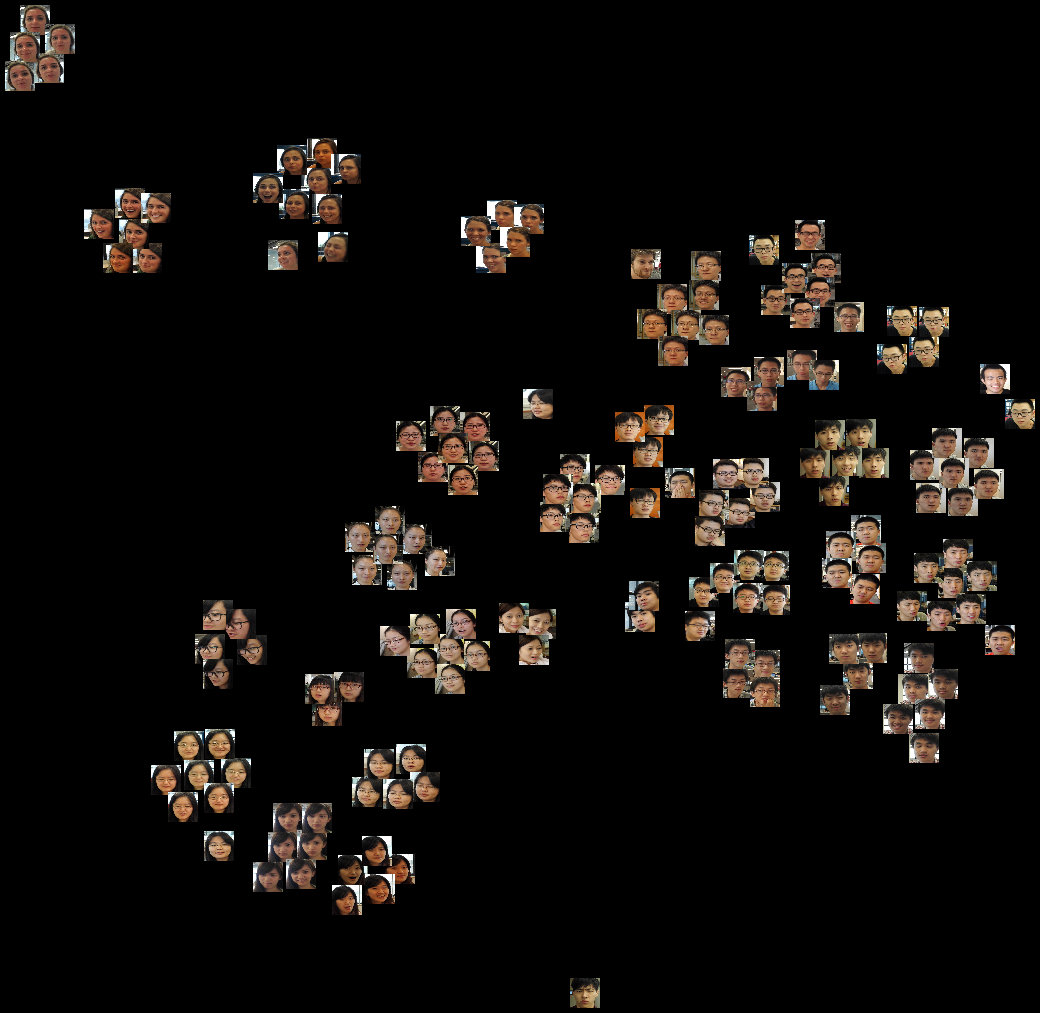
\includegraphics[width=0.6\textwidth]{figure/ch4-tsnevggfc8.png}}
        \raisebox{-0.5\height}{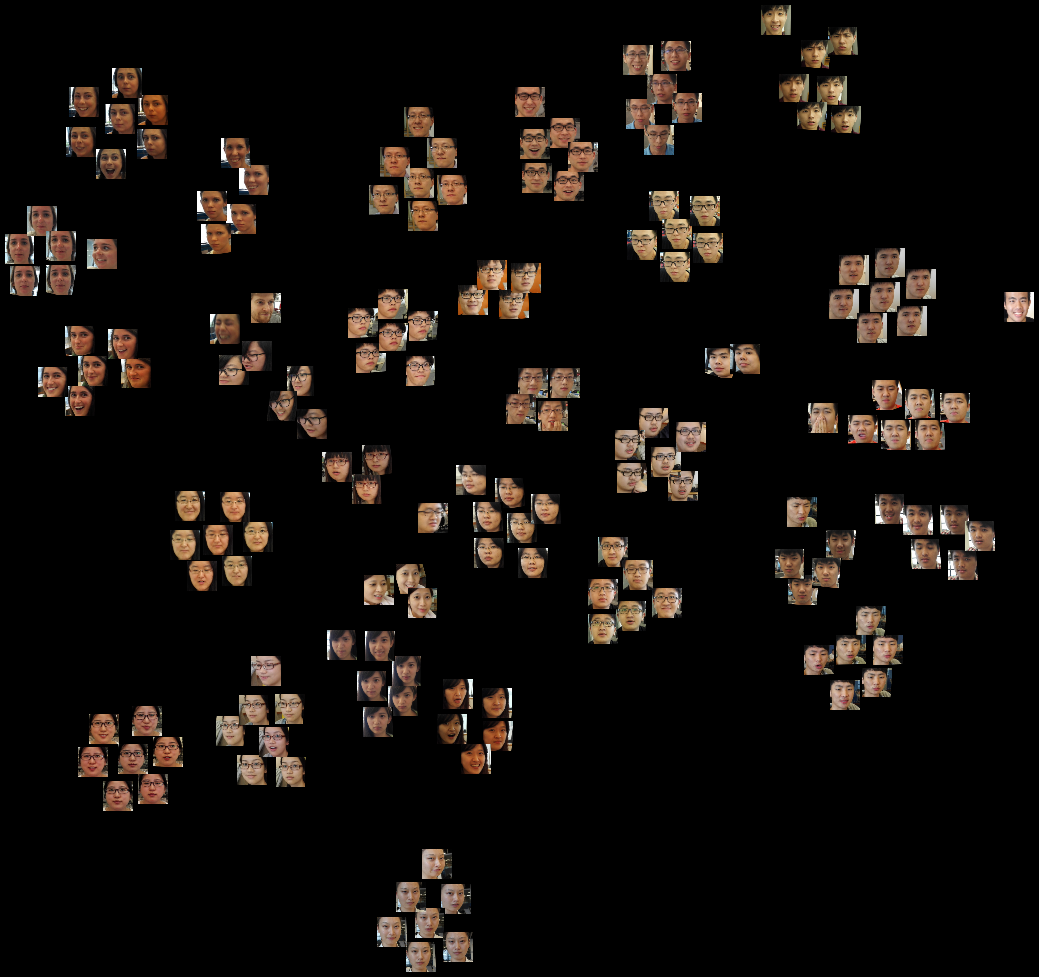
\includegraphics[width=0.62\textwidth]{figure/ch4-tsnemfmeltwise_fc1.png}}
    }
    \caption{t-SNE visualization of VGG \emph{fc8} layer features and Lightened CNN \emph{fc1} layer features.}
    \label{fig:ch4-tsnevggvsmfm}
\end{figure}

To compare performance of features extracted from the two models, we run t-SNE visualization~\cite{maaten2008visualizing} on the features of a small dataset we previously collected for emotion sensing. Fig~\ref{fig:ch4-tsnevggvsmfm} shows the t-SNE visualization result. It seems VGG feature and Lightened CNN feature have similar performance, at least on this small dataset. Though it is found that comparing to Lightened CNN model, VGG model is more robust to variations and its features show better transferability~\cite{ghazi2016comprehensive}, the model size is more than 500MB, 10 times bigger than Lightened CNN model. And the released VGG model has a feature dimension of 4096, while Lightened CNN model has a feature dimension of 256. Our experiment on different Android smartphones shows it takes 10 times longer to extract VGG features. Table~\ref{tbl-forwardingtime} shows the forwarding time we tested on different smartphones. It can be seen VGG model consumes much more memory that it can only run on phones with memory larger than 3GB. Due to above concerns, we use Lightened CNN model in our implementation.

\begin{table}[!htbp]
\centering
\caption{Time of single facial feature extraction and batch facial feature extraction (10 faces).}
\label{tbl-forwardingtime}
\begin{tabular}{lrrr}
\toprule
 & Xiaomi Mi 3W & Galaxy Note 4 & Xiaomi Mi 5\\
 & {\small Snapdragon 800} & {\small Snapdragon 805} & {\small Snapdragon 820}\\
 & {\small 2GB RAM} & {\small 3GB RAM} & {\small 4GB RAM}\\
 \midrule
1 VGG CNN & N/A & N/A & $\sim 2780$ ms \\
10 VGG CNN & N/A & N/A & $\sim 26740$ ms \\
1 Lightened CNN & $\sim 508$ ms & $\sim 330$ ms & $\sim 303$ ms \\
10 Lightened CNN & $\sim 6602$ ms & $\sim 3971$ ms & $\sim 2031$ ms \\
 \bottomrule

\end{tabular}
\end{table}


\subsubsection{Detection and Alignment}
Lightened CNN model takes aligned face as input, requiring that the distance between midpoint of eyes and midpoint of mouth is 48, and $y$ value of midpoint of eyes is 40, as shown in Fig~\ref{fig:ch4-facedetalign}. We use OpenCV's haar cascade~\cite{links:opencv,viola2001rapid} frontal face detector. The limitation it brings to Cardea is only frontal faces will be detected and recognized. We set \emph{minNeighbors} (the parameter specifying how many neighbors each candidate rectangle should have to retain it) to be 3 to ensure a relative high recall for face detection. To remove false positive, we further apply skin color filter (range $[0, 48, 60] - [30, 255, 255]$ in HSV color space) on retained rectangles. Following that, we use Dlib library's HOG~\cite{links:dlib,dalal2005histograms} based face detector as a second stage filter. Note that Dlib's face detector has higher accuracy comparing to OpenCV's face detector, but is much slower if applied directly on a high resolution image, therefore it is used as a filter on small rectangular areas. Dlib's facial landmarks detector~\cite{links:dlibfacepose} is also used in later face alignment stage, it can detect 68 facial landmarks~\cite{links:dlibfacelandmarkspos, links:dlibfacelandmarkscoords}. With the detected landmarks and required alignment condition about inputs to the CNN model, we can calculate the homography matrix that is finally used to align faces. The steps for detection and alignment is shown in Fig~\ref{fig:ch4-facedetalign}, and we implemented it as a JNI library for Android platform~\cite{links:facealignjni}.

\begin{figure}[!htbp]
    \centering
    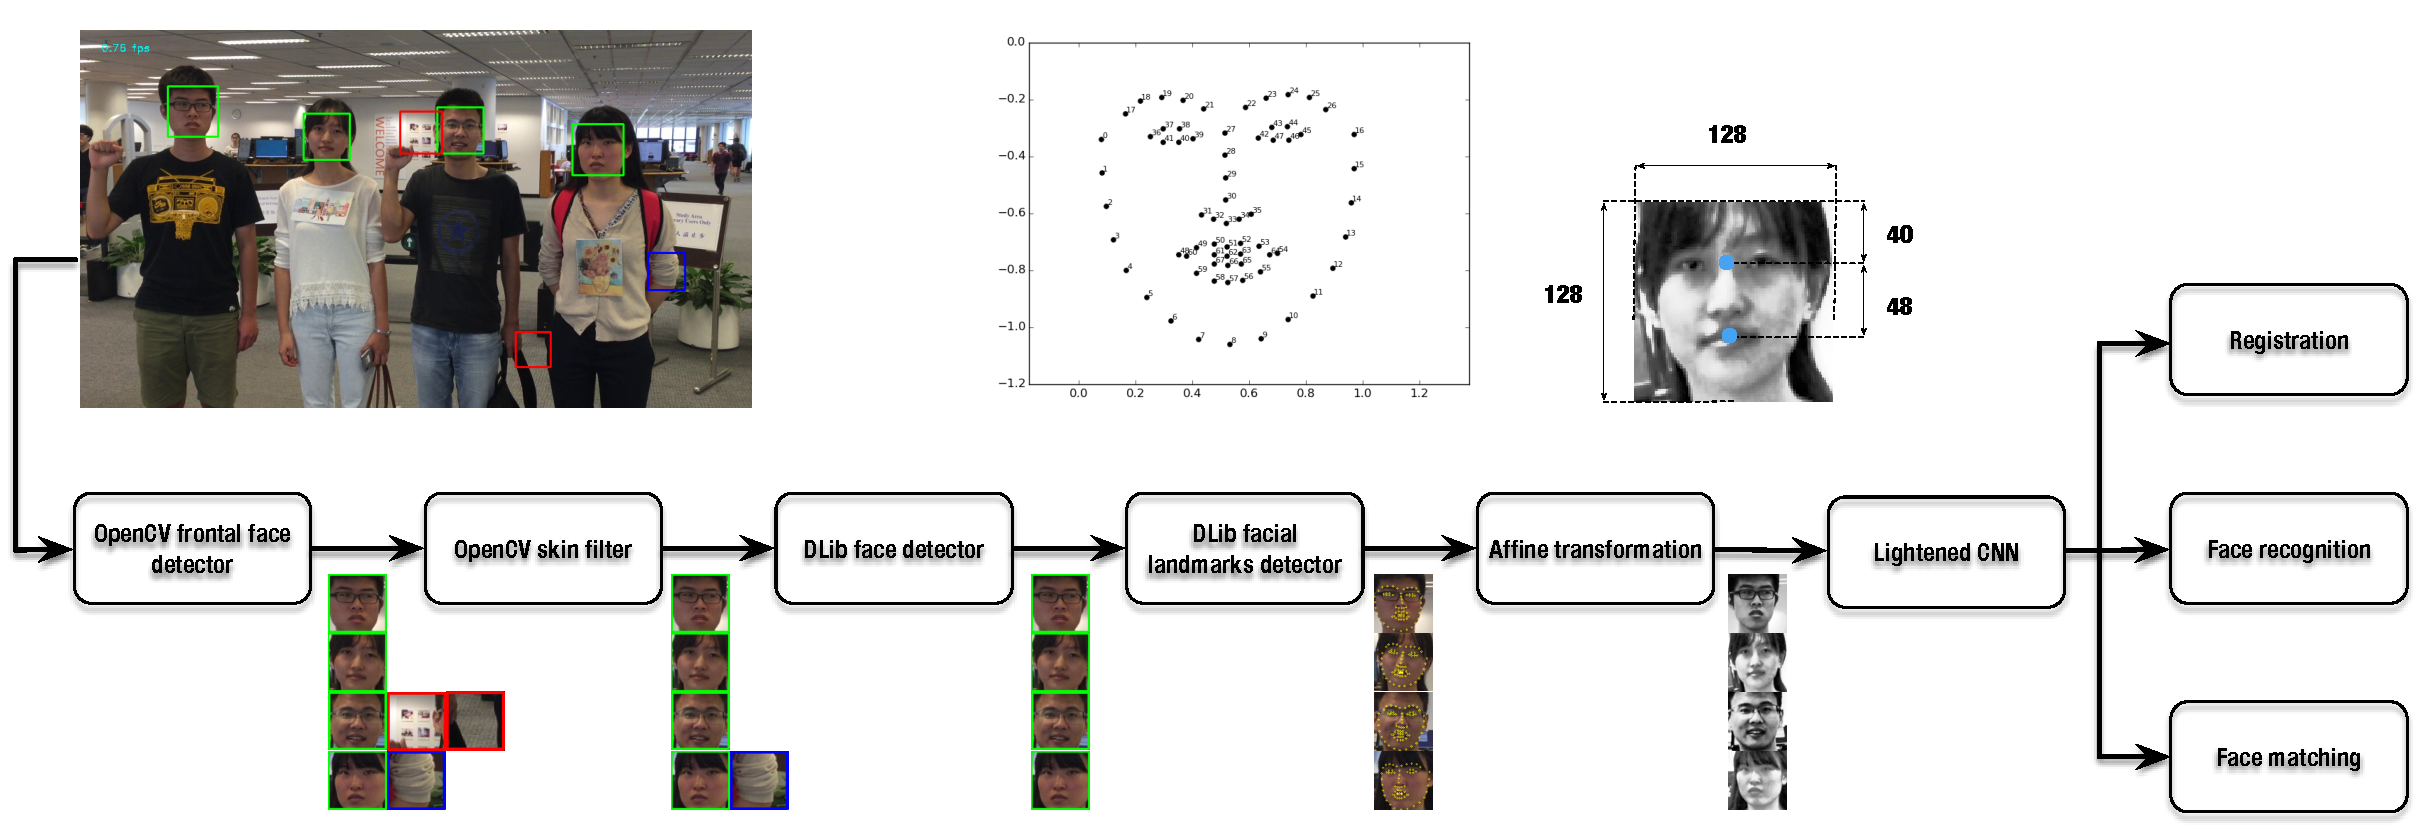
\includegraphics[width=1.0\textwidth]{figure/ch4-facedetalign.pdf}
    \caption{Face detection and alignment workflow.}
    \label{fig:ch4-facedetalign}
\end{figure}

\subsubsection{Recognition}
All the facial features uploaded by registered users are used to train a classifier in the cloud server, using LIBSVM library~\cite{chang2011libsvm}. During training, we set the parameter to enable probability estimations of classes $p_i, i\in{1, \cdots, N}$. In prediction time for each facial feature, if $\max_ip_i \leq 0.3$, then we treat it as from an unknown person who hasn't registered in Cardea, otherwise it is from the user who has the highest probability and his privacy preference will be fetched for further processing.

\subsubsection{Matching}
Face matching occurs when a recognized user $A$ has also specified and uploaded features of person $B$ with whom he doesn't want to be captured, it is to determine whether $B$ also appears in this captured image. Note that $B$ is not necessarily a registered user of Cardea. It is required that $N_B$, the number of $B$'s facial features uploaded by $A$ should be more than $10$. Then feature $f_l$ from other faces $l\neq A$ in the image will be compared with $B$'s features. $\mathtt{Cosine}$ similarity is used as distance metric. Among $N_B$ distances between $f_l$ and $B$'s features, we can calculate the ratio $r$ of distances which are shorter than a threshold $d_ \mathit{threshold}$, if the ratio $r$ is higher than a threshold $r_ \mathit{threshold}$, then $l$ and $B$ are the same person, thus $B$ appears with $A$ in the same image. By tuning, we find $d_ \mathit{threshold} \in (0.3, 0.5)$ and $r_ \mathit{threshold} \in (0.5, 0.8) $ shows good enough performance. In Fig~\ref{fig:ch4-mfmsim}, we plot the distribution of distance between same person's Lightened CNN features and different person's Lightened CNN features. The features are extracted from all the faces in ORL face database~\cite{links:orlfacedb}, which consists of 400 images from 40 distinct subjects, 10 images per subject. Each subject has different photos, such as: with/without glasses, open/closed eyes, and different facial expressions. It is obviously seen that distances between same person and different persons are well seprated, especially for the case of $\mathtt{cosine}$ similarity.

\begin{figure}[!htbp]
    \centering
    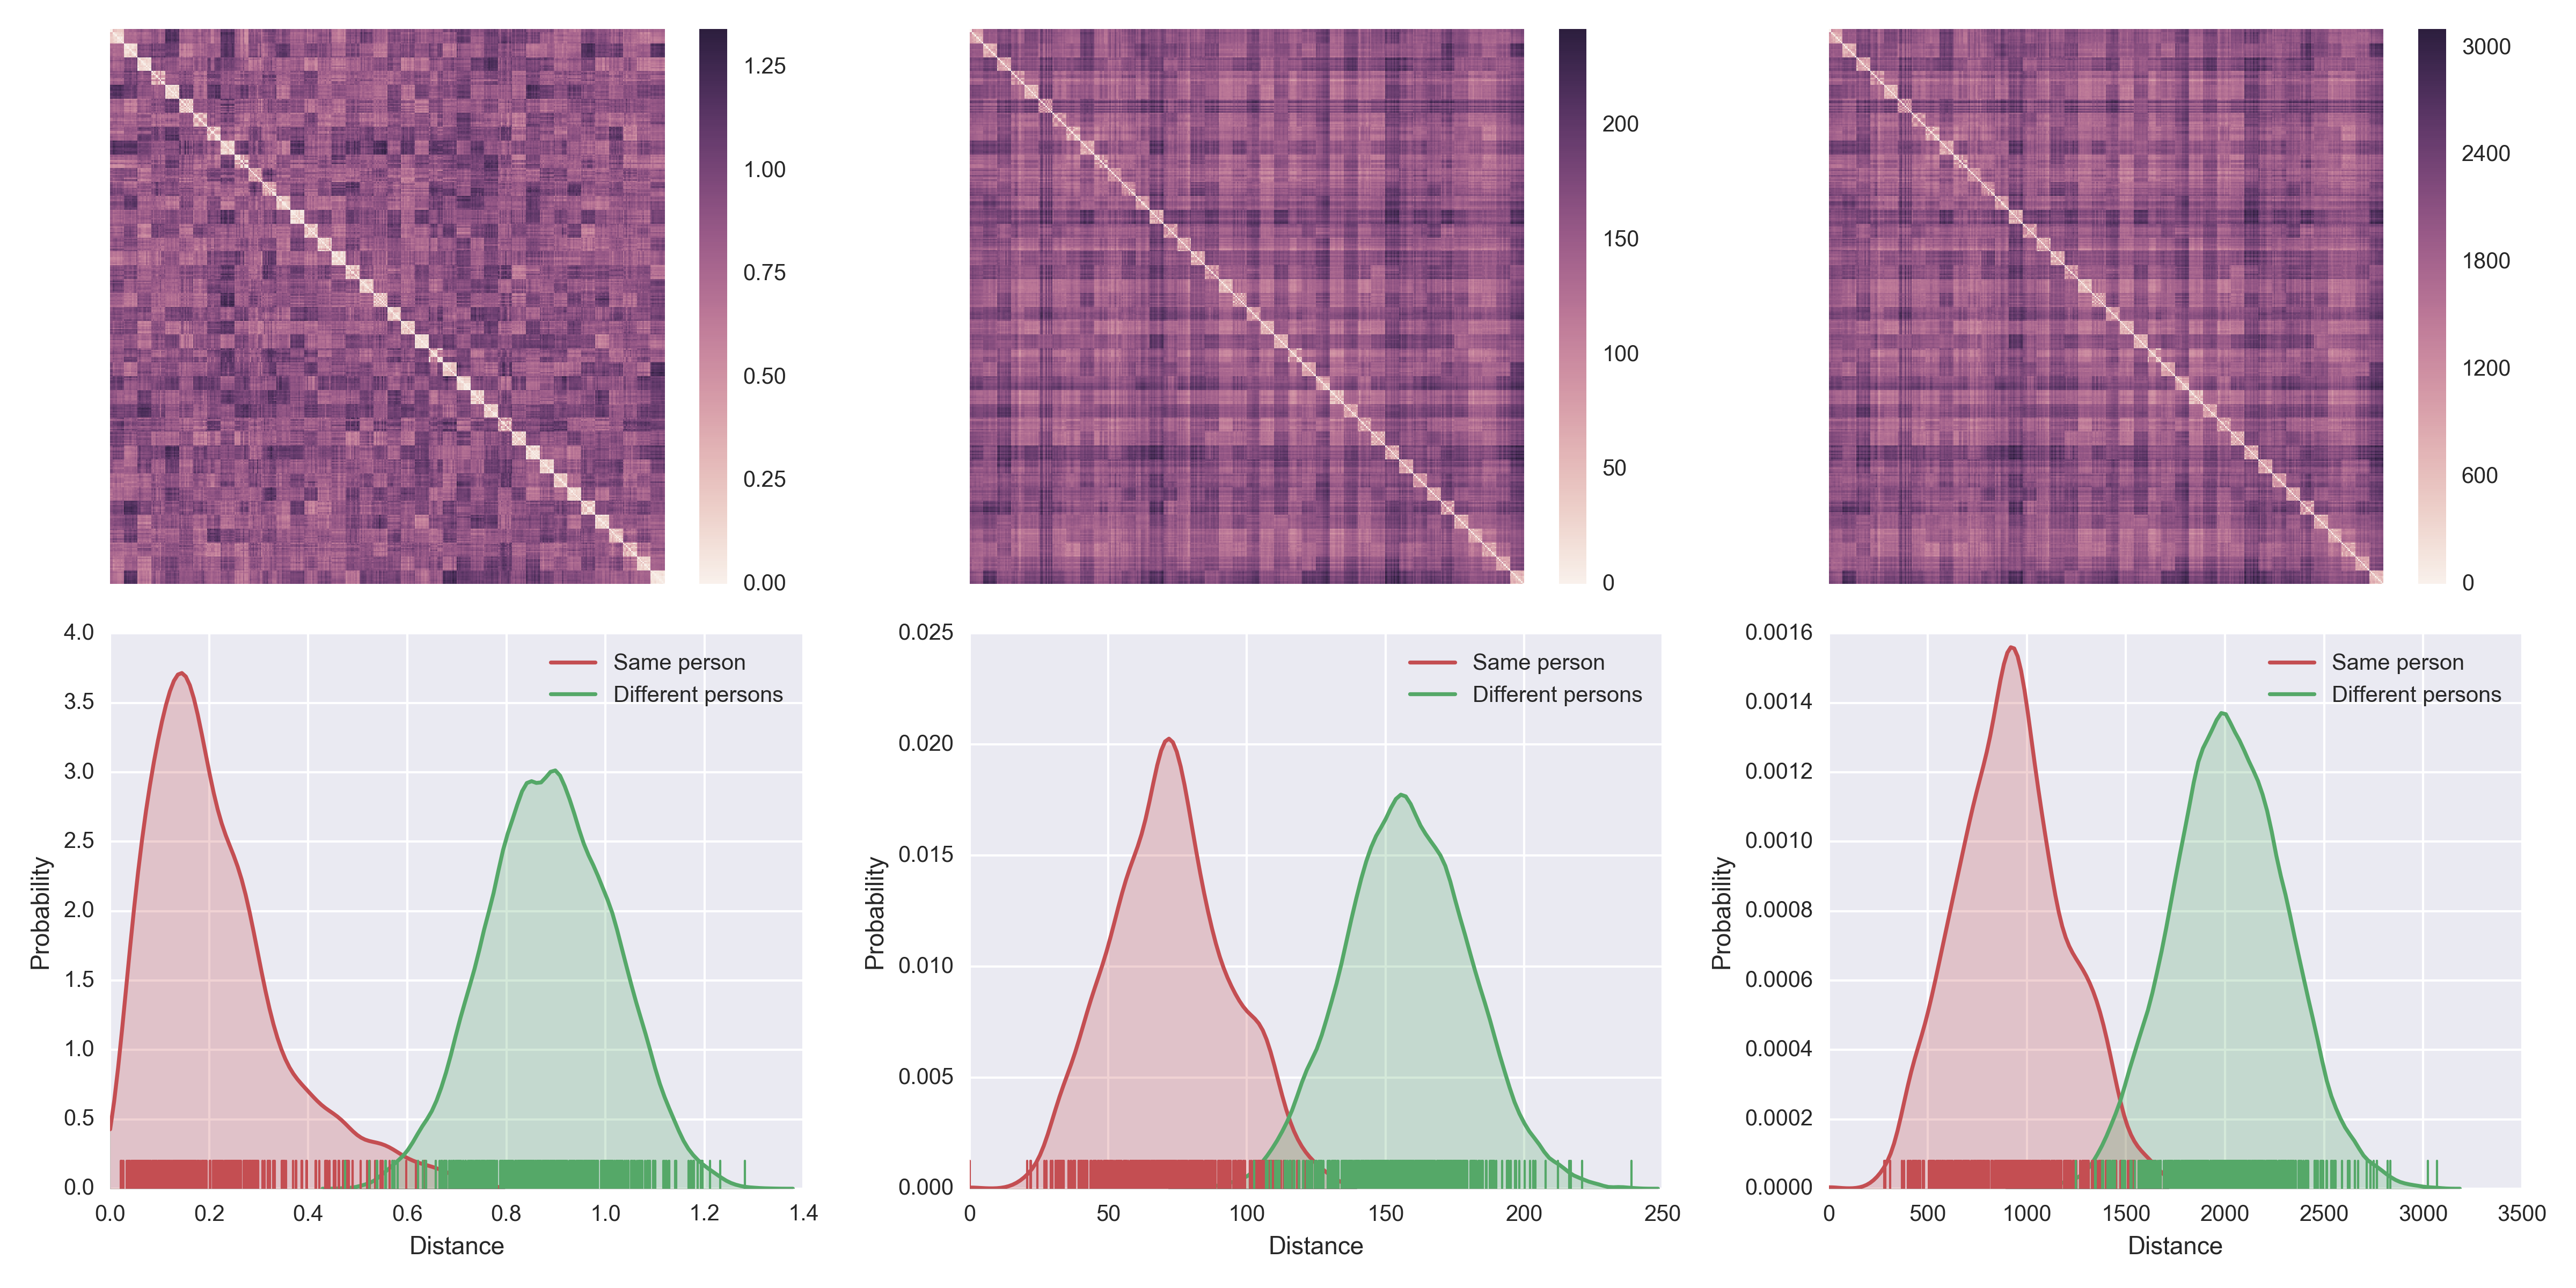
\includegraphics[width=1.0\textwidth]{figure/ch4-mfmsim.png}
    \caption{Distance matrix (top) and distance distribution (bottom) of Lightened CNN features using $\mathtt{cosine}$ similarity (left), $l_1$ norm (center) and $l_2$ norm.}
    \label{fig:ch4-mfmsim}
\end{figure}


\subsection{Gesture Recognition}
In Cardea, "yes" (\vcenteredinclude{figure/ch4-yesgesticon.png}) and "no" (\vcenteredinclude{figure/ch4-nogesticon.png}) gestures have the highest priorities and are used to temporarily overwrite privacy preferences. To recognize gestures in daily life images, the first step is detection of hands, and it turns out to be the most challenging part in this sub task. Skin color based hand detector will fail dramatically in images with cluttered background. A much more robust method will be using multiple proposals~\cite{mittal2011hand} based on hand shape, context, and skin color. However, it takes an extremely long time to detect hands in one image. Finally, we choose to leverage state-of-the-art detection framework faster R-CNN~\cite{ren2015faster} to train a gesture detector in an end-to-end manner.

\subsubsection{Data Preparing and Preprocessing}


VGG group has shared a comprehensive dataset of hand images collected from various different public image data set sources in~\cite{mittal2011hand, links:vgghanddataset}. It contains 5628 images, which is composed of 4069 training images, 738 validation images, 821 testing images respectively, each image is with annotations of hand bounding boxes. However, this dataset can only let us train a hand detector. To achieve the goal of recognizing gestures, there are two solutions in our consideration:

\begin{itemize}
\item First train a hand detector using this dataset, then train another hand gesture classifier using other commonly used gesture datasets and pipe them together.
\item Take this dataset as a subset of images with "natural" gestures, then prepare extra images with "yes" and "no" gestures including annotations by ourselves, and train a "natural/yes/no" gesture detector end-to-end.
\end{itemize}

The first solution is not an end-to-end solution, and the specific "yes" and "no" gestures may not be included in those standard gesture datasets, then we will still need to prepare our specific gesture dataset like in second solution. Therefore, we choose the second solution, based on the observation and also assumption that annotated hands in VGG's hand dataset are in natural relaxing modes, thus will not be treated as "yes" or "no" gestures. The annotations of VGG dataset are tilted rectangles shown as yellow ones in Fig~\ref{fig:ch4-gesturedataset}, we re-annotate the dataset using bounding boxes of the original annotations shown as blue rectangles.

We crawled 527 images with "yes" hand gestures, and 363 images with "no" hand gestures. Note that in a crawled image, it may contain different types of hand gestures as shown in Fig~\ref{fig:ch4-gesturedataset}, which is not a problem so long as gesture types are annotated correctly (\emph{remind} that all gestures in VGG dataset are treated as "natural" class). These images are crawled from Google and Flickr image search with keywords such as "victory sign", "stop gesture", "palm gesture" and so on, many of them are focused on the hands thus don't contain many background pixels. We rescale these images in different scales and then pad zeros on rescaled images. In Faster-RCNN python implementation~\cite{links:pyfasterrcnn}, an input image is rescaled to around $1000\times 1000$ before fed to region proposal network. If without padding data augmentation step, the bounding boxes of hand gestures will be huge in many crawled images that are focused on hands, which makes the learned model not able to detect small hand gestures and also not perform well on the regression of large hand gestures. Another reason for the padding step is to counter data imbalance of three classes. After augmentation, we have a dataset of 13843 images, including 5628 images from VGG dataset, 4712 augmented images mostly with "yes" gestures and 3503 augmented images mostly with "no" gestures. Fig~\ref{fig:ch4-gesturedataset} shows some sample images with annotations from this composed dataset. We wrote a tool~\cite{links:imgannota} to annotate the crawled images.

\begin{figure}[!htbp]
    \centering
    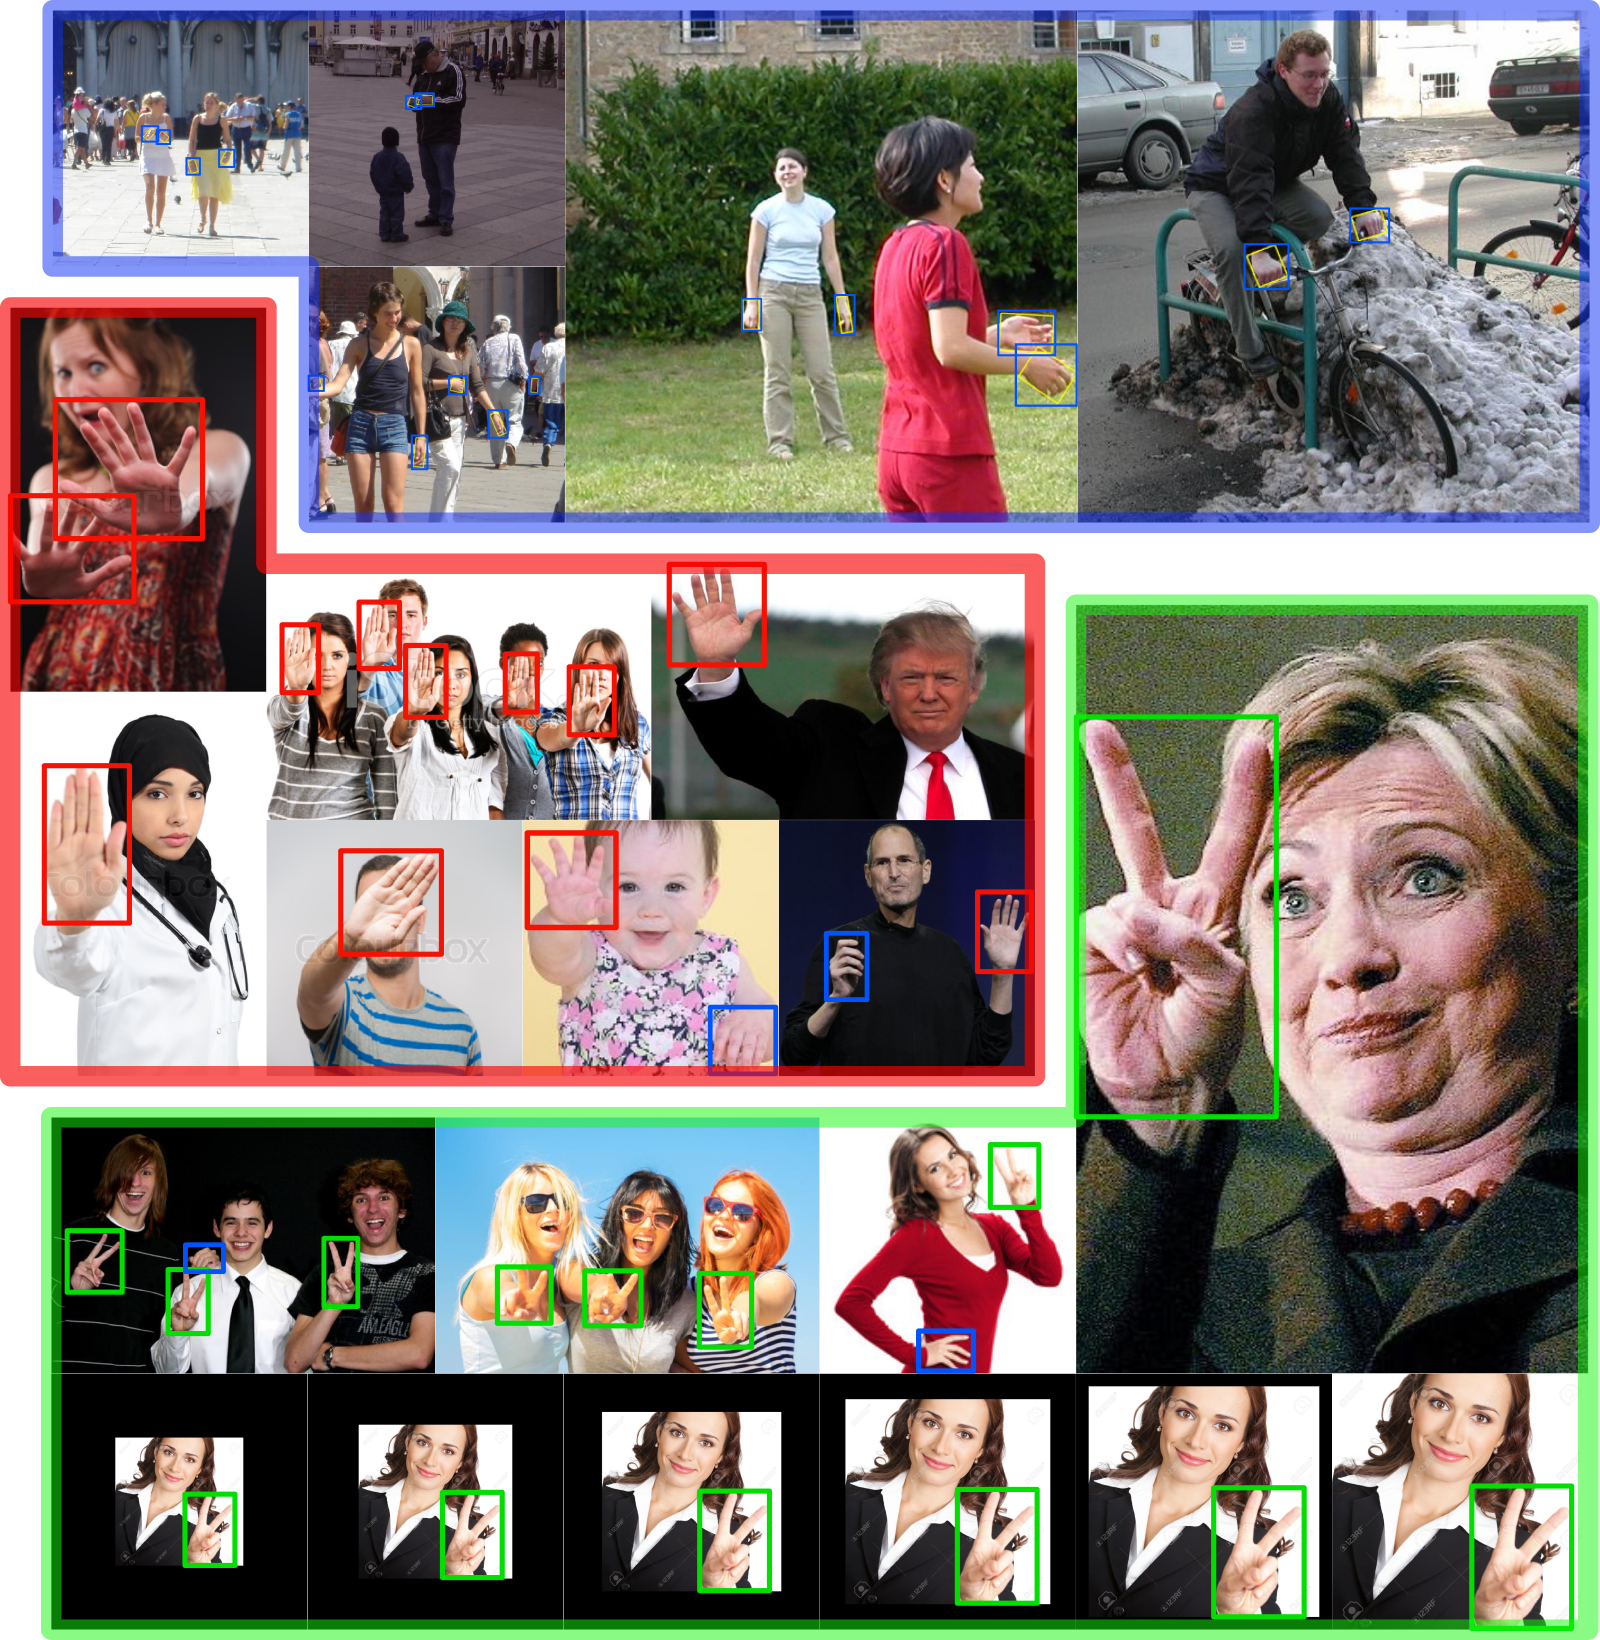
\includegraphics[width=0.8\textwidth]{figure/ch4-gesturedataset.png}
    \caption{Training hand gesture dataset composed of VGG hand dataset (blue) and augmented crawled dataset (red and green).}
    \label{fig:ch4-gesturedataset}
\end{figure}

\subsubsection{Training Procedures}
Using the composed dataset, we fine-tune the \emph{conv3\_1} and up layers of VGG16 pre-trained model provided by Faster-RCNN library, jointly with region proposal layers and detection layers that are not part of VGG16 pre-trained model. Features from \emph{conv5\_3} layer of VGG16 network are shared by region proposal network (RPN) and Fast-RCNN~\cite{girshick2015fast} detection network, RPN uses them to generate proposals, and region of interest (ROI) pooling layer in detecting network uses them for bounding box regression and classification. There are two methods to train a shared feature extraction network. One is an alternating optimization method with following steps: \ding{182} Train an RPN $M_1$ initialized from VGG16 pre-trained model $M_0$, \ding{183} Generate training proposals $P_1$ using RPN $M_1$, \ding{184} Train Fast R-CNN model $M_2$ on proposals $P_1$ initialized from $M_0$, \ding{185} Train RPN $M_3$ from $M_2$ without changing convolutional layers, \ding{186} Generating proposals $P_2$ using RPN $M_2$, \ding{187} Train Fast R-CNN model $M_4$ on proposals $P_2$ initialized from $M_3$ without changing convolutional layers, \ding{187} Add $M_3$'s RPN layers to Fast R-CNN model $P_2$. Another method is an approximate joint optimization method by training with stochastic gradient descent as usual, which is easier, faster and achieves similar performance~\cite{links:pyfasterrcnn}, so we use the second training procedures.

\subsubsection{Prediction}
During prediction, we set Non-Maximum Suppression (NMS) threshold as 0.4 and confidence level threshold as 0.7. Figure~\ref{fig:ch4-gestpredictemp} shows some examples of gesture detection and recognition results in natural environment. It can be seen that the trained model can handle cluttered background such as in shopping environment, and indoor dark lighting condition. It is interesting to notice that bounding boxes for "natural" hands are bigger, reflecting the fact that we select re-annotated the VGG dataset for "natural" class using bounding boxes of the original annotations. The model has a good recall in terms of hand detection, however, its gesture recognition is sensitive to motion blur, palm angles and gesture size. We think the good recall of hands comes from the comprehensive VGG dataset, and the not so good recognition result is because the "yes/no" dataset we composed does not have a good quality because gestures are focused in many images, especially for "no" gestures, which is reflected by the observation that "yes" gesture recognition performs better than "no" gesture.

\begin{figure}[!htbp]
    \centering
    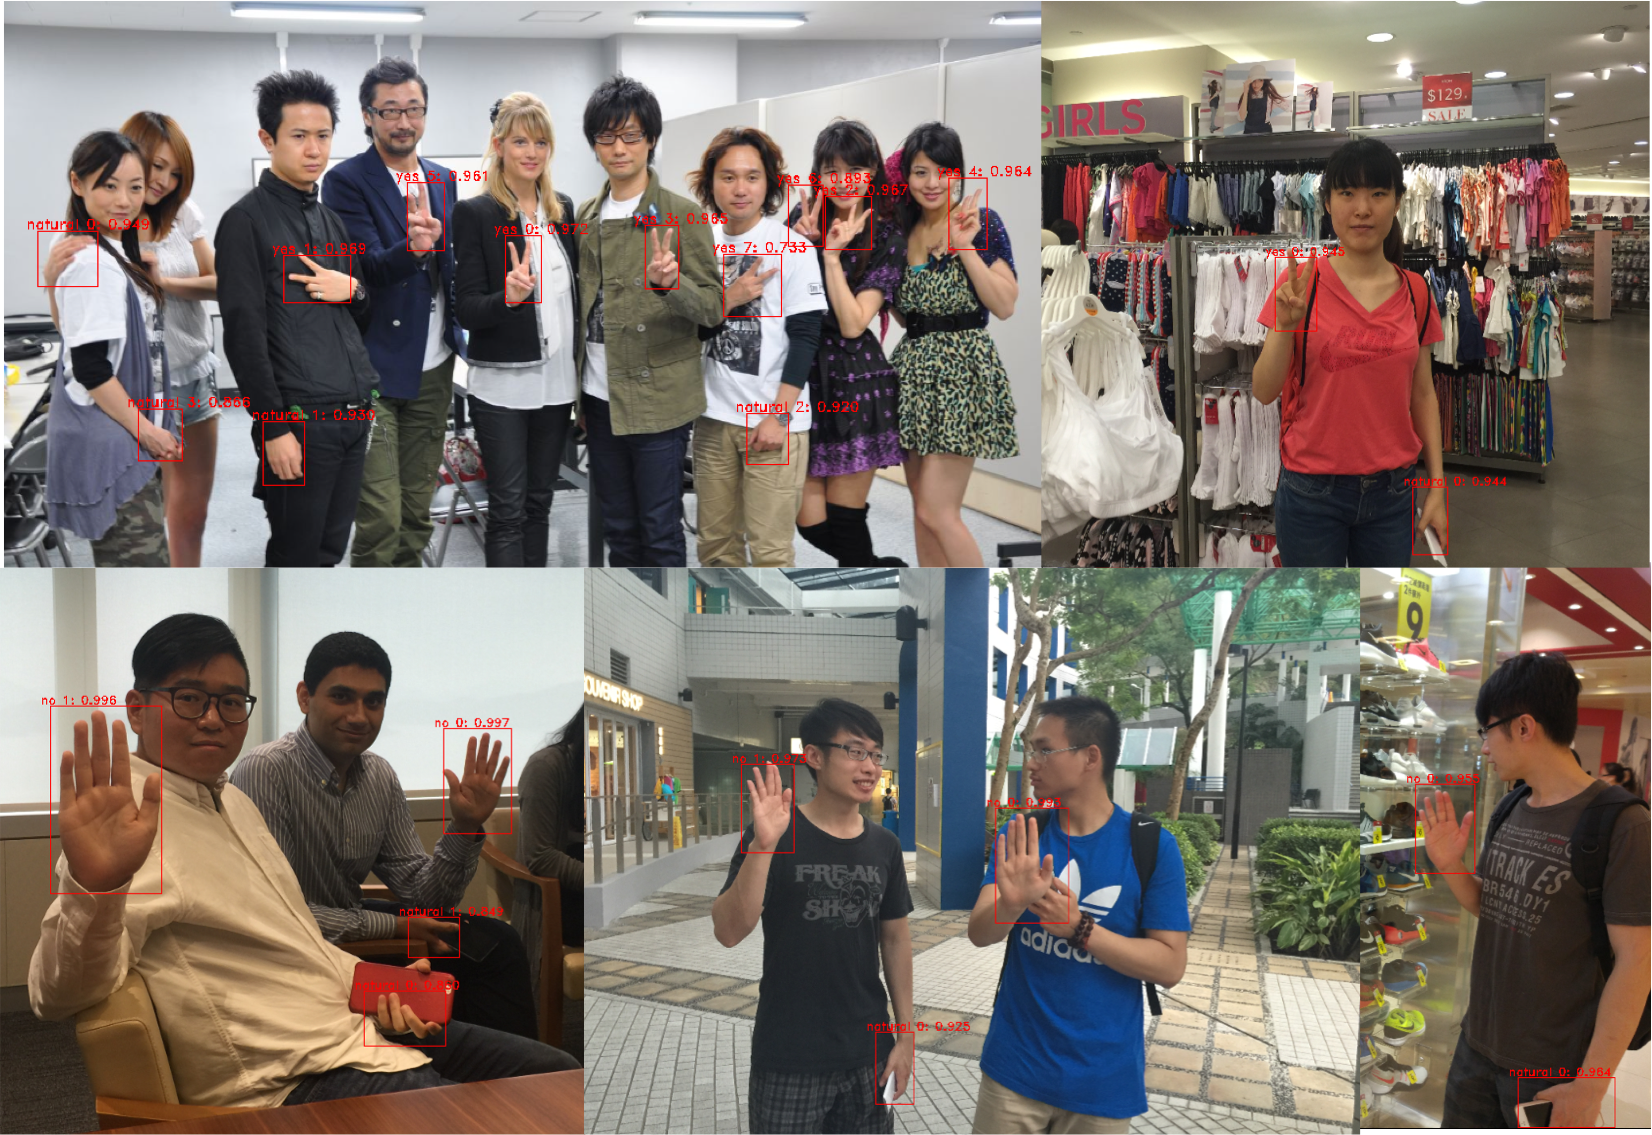
\includegraphics[width=0.8\textwidth]{figure/ch4-gestpredemp.png}
    \caption{Examples of gesture detection and recognition.}
    \label{fig:ch4-gestpredictemp}
\end{figure}



\section{System Integration}

\subsection{Deployment on Android}

Ideally, for a privacy control framework, we prefer a design that does not require cloud server and all the algorithms run locally on mobile devices. In the current design and implementation, cloud server exists mainly for two reasons: \ding{182} Storage center for profiles and hosting face recognition model; \ding{183} RPN in gesture recognition task is written in Python language, thus gesture recognition can not run on Android smartphones easily. However, these are not hard restrictions, possible improvements are discussed in Chapter 5.

The deployment of Caffe models for scene classification and facial feature extraction is based on Caffe-android-library~\cite{links:caffeandroidlib}, we modified its code~\cite{links:caffeandroidlibzr} to support loading multiple Caffe models, batch feature extraction, and only forwarding to a specified layer during feature extraction, which saves useless computations from fully connected layers. There are other libraries for deploying neural networks on mobile, such as Torch-android~\cite{links:torchandroid} and MXNet~\cite{links:mxnetmobile}. The deployed scene classification model (based on AlexNet structure) has a size of 230MB, which is not small. However, its prediction is very fast, and can be easily fitted into the time slot of waiting response from cloud server. The facial feature extraction model (based on Lightened CNN structure) has a relatively bearable size of 33MB. Comparing to AlexNet, Lightened CNN model has smaller filter sizes, but with many more feature maps, therefore in run time, Lightened CNN model consumes about 1GB memory, which makes it not able to run on smartphones with less than 2GB memory~\ref{tbl-forwardingtime}. Possible ways to decrease model size and optimization of resource consumptions are also discussed in next chapter. Other lighter models we deployed on android include OpenCV face cascading model (less than 1MB), and shape predictor (90MB) in Dlib facial landmark detection.


\begin{figure}[b!]
    \centering
    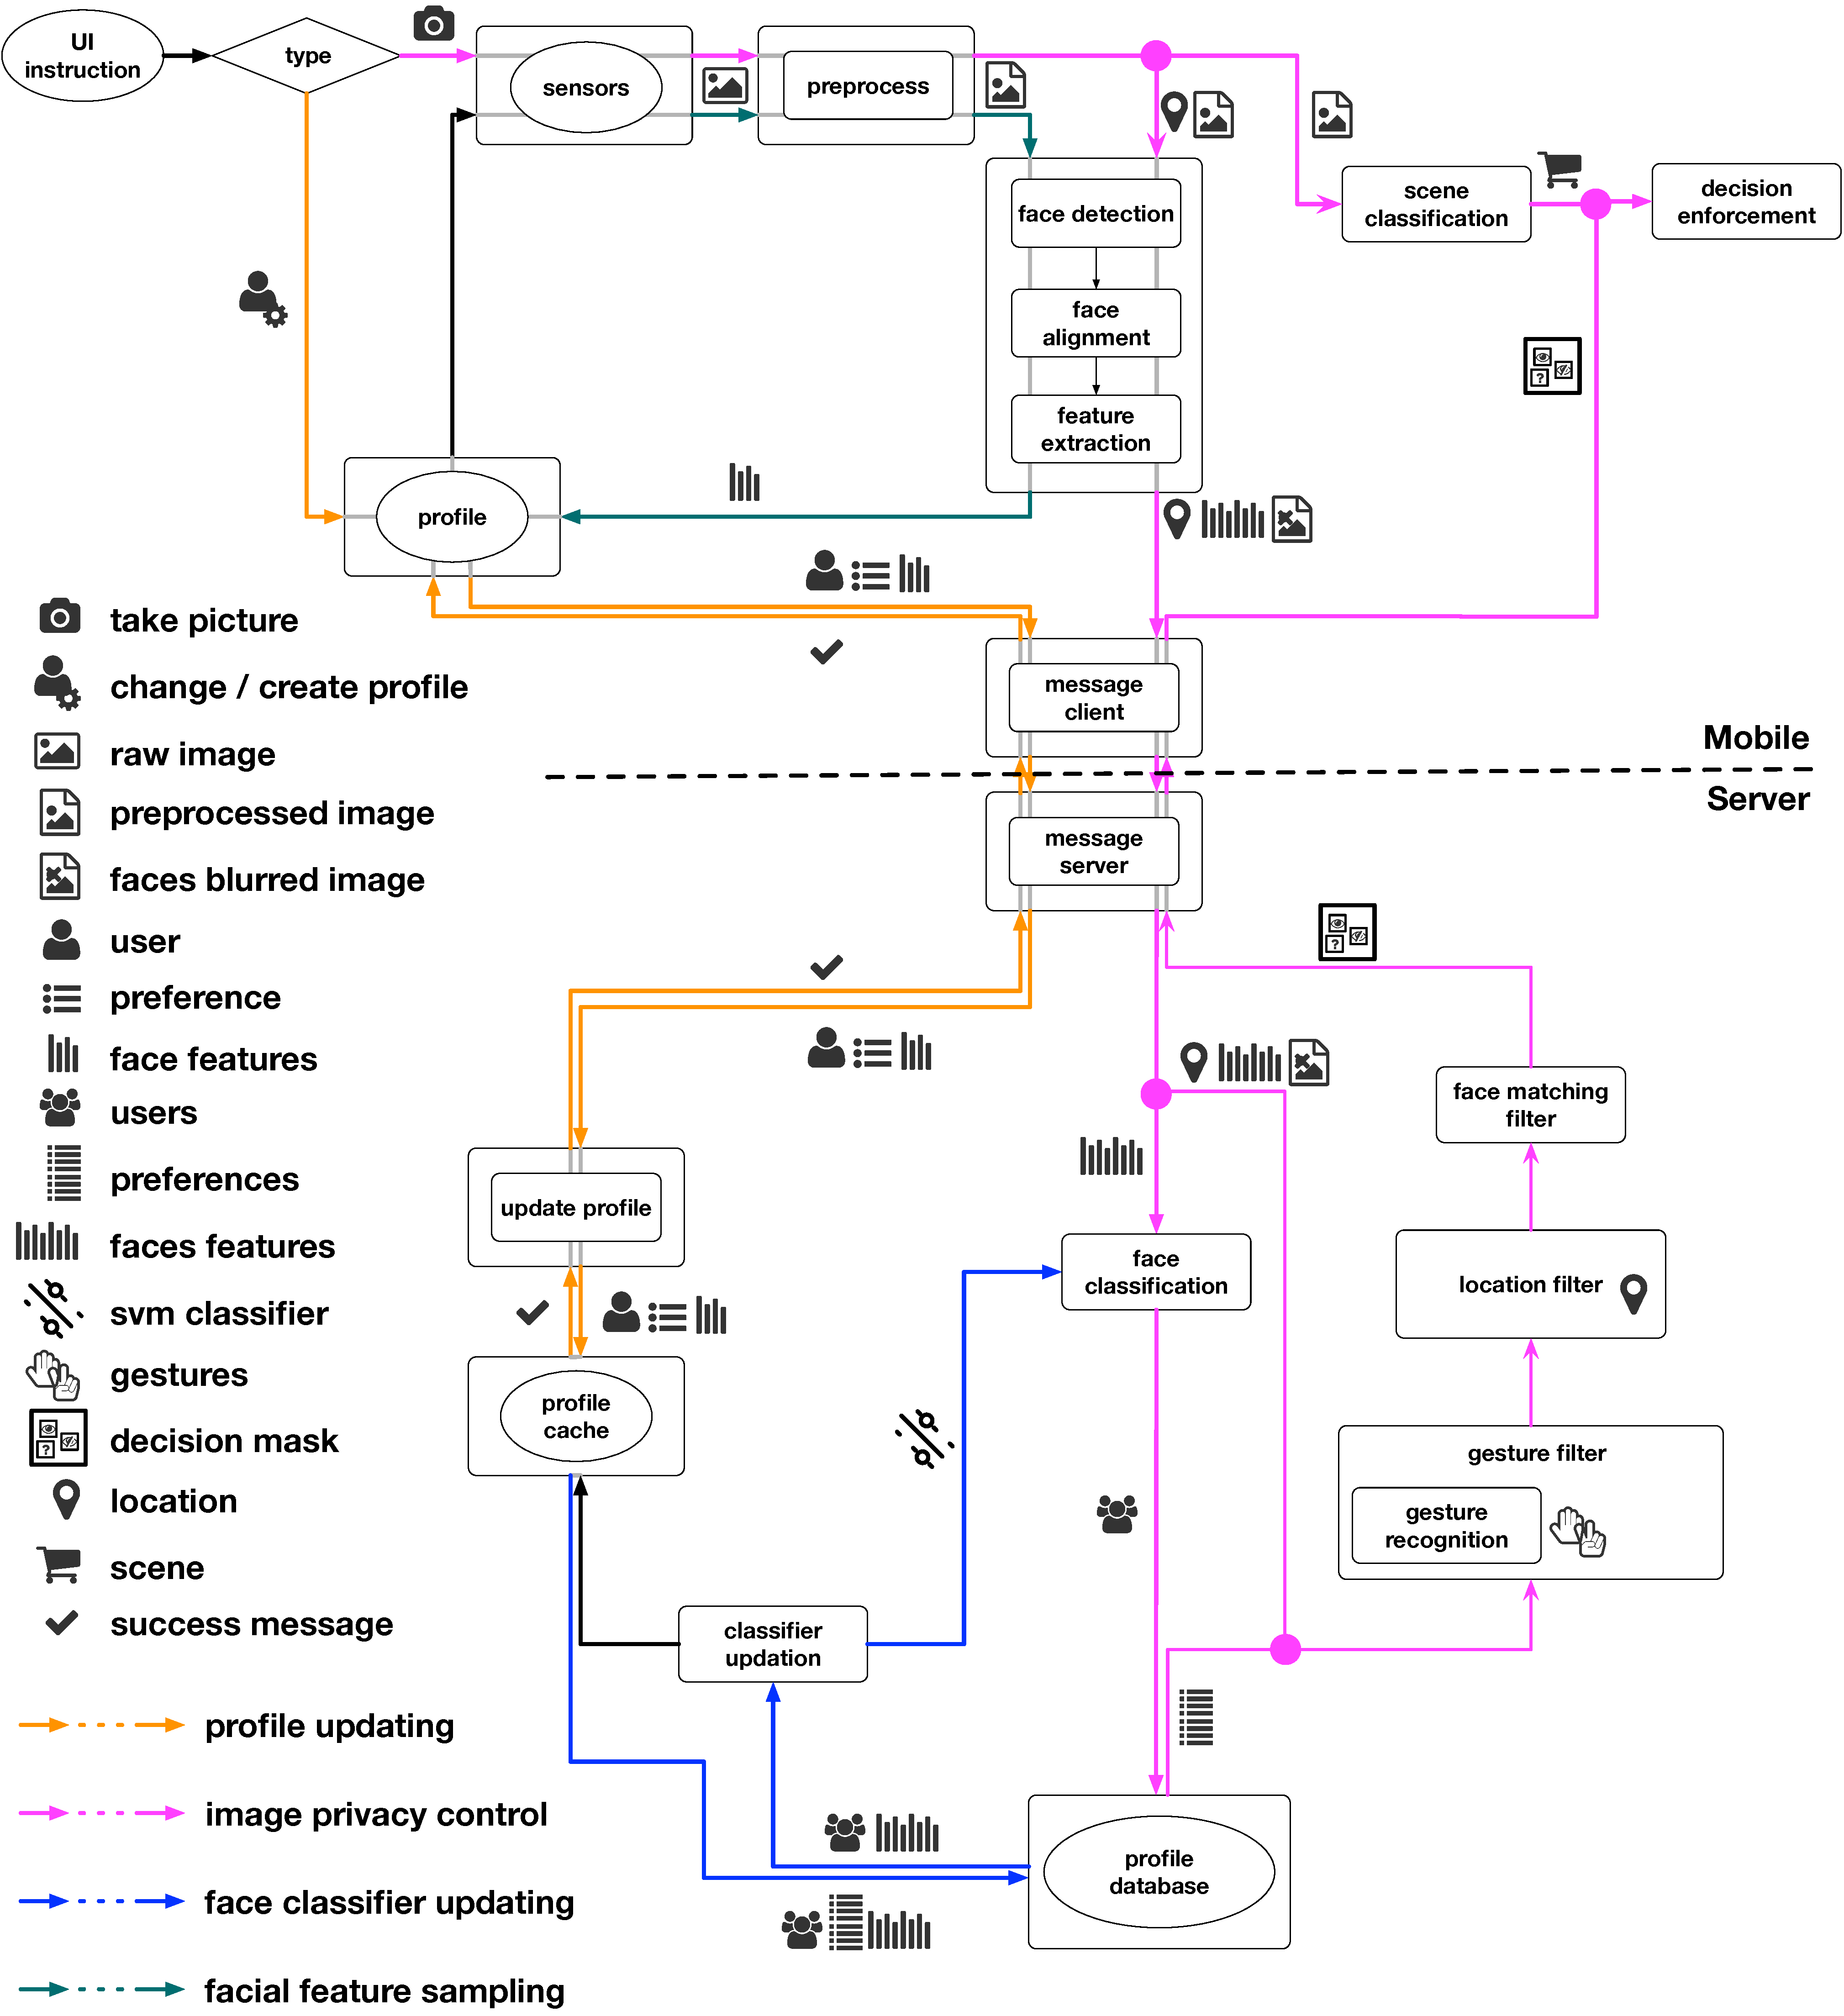
\includegraphics[width=0.6\textwidth]{figure/ch4-cardeadataflow.pdf}
    \caption{Dataflow of Cardea}
    \label{fig:ch4-cardeadataflow}
\end{figure}

\subsection{Dataflow and Integration}
Fig~\ref{fig:ch4-cardeadataflow} shows the detailed structure and dataflow of Cardea, which is mainly composed of the following steps (a demo video about the usage can be found in~\cite{links:cardeavid}):

\begin{description}[leftmargin=0cm]

\begin{figure}[!htbp]
    \centering
    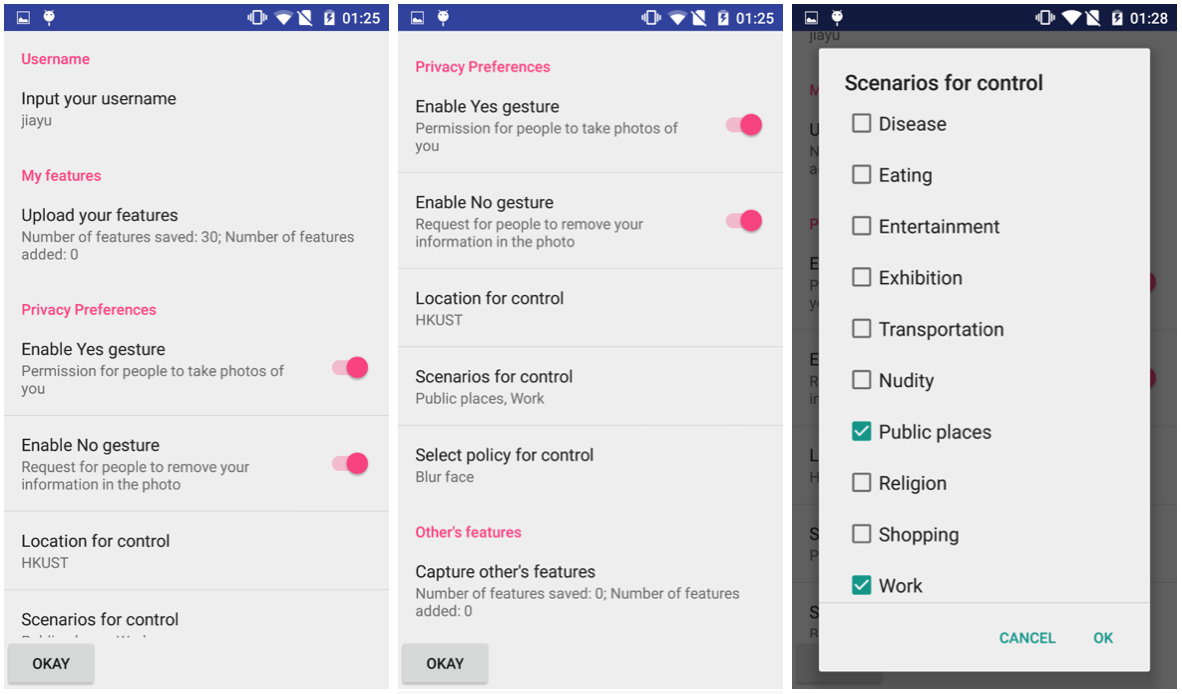
\includegraphics[width=0.6\textwidth]{figure/ch4-reg.png}
    \caption{Registration and profile updating interface}
    \label{fig:ch4-reg}
\end{figure}

  \item[{Registration and Profile updating:}] The interface of registration for bystanders and updating of profiles is shown in Fig~\ref{fig:ch4-reg}. He is able to select one or more scene categories, one location for control, as well as enable gestures or not. In two cases his facial features will be packaged with his privacy preferences: one is in registration time and the other is when he wants to update his facial features in the cloud. This registration and updating message will be send to server, if it is an updating message without feature updating, then his user profile in cloud will be updated immediately and he will receive a "success" notification, otherwise this message will be first buffered in a profile cache.

  \item[{Face classifier updating:}] In the server, the face classifier will be updated intermittently. For every time interval $\Delta T$, if there is cached messages that brings new facial features, it will \ding{182} block the queue of prediction messages from doing face recognition, \ding{183} merge profile cache with profile database, \ding{184} retrain a face classifer and \ding{185} unblock queued prediction messages.

  \item[{Image capturing:}] When a recorder uses Cardea to take a image, extracted facial features, GPS coordinate as well as face-blurred image will be packaged as prediction message and sent to server for processing. In the server side, after faces recognition and profiles retrieval, it will start the cloud part of decision making process for every bounding box, returned to the client side is a decision mask that specifies among all the detected faces, which should be blurred, which should be kept and which should be further determined based on the scene results calculated on the client side. In client side, while waiting for response from server it will calculate the scene result. With received decision mask, it makes final decisions on every face and enforces the privacy protection actions complied with everyone's preference.

\begin{figure}[!htbp]
    \centering
    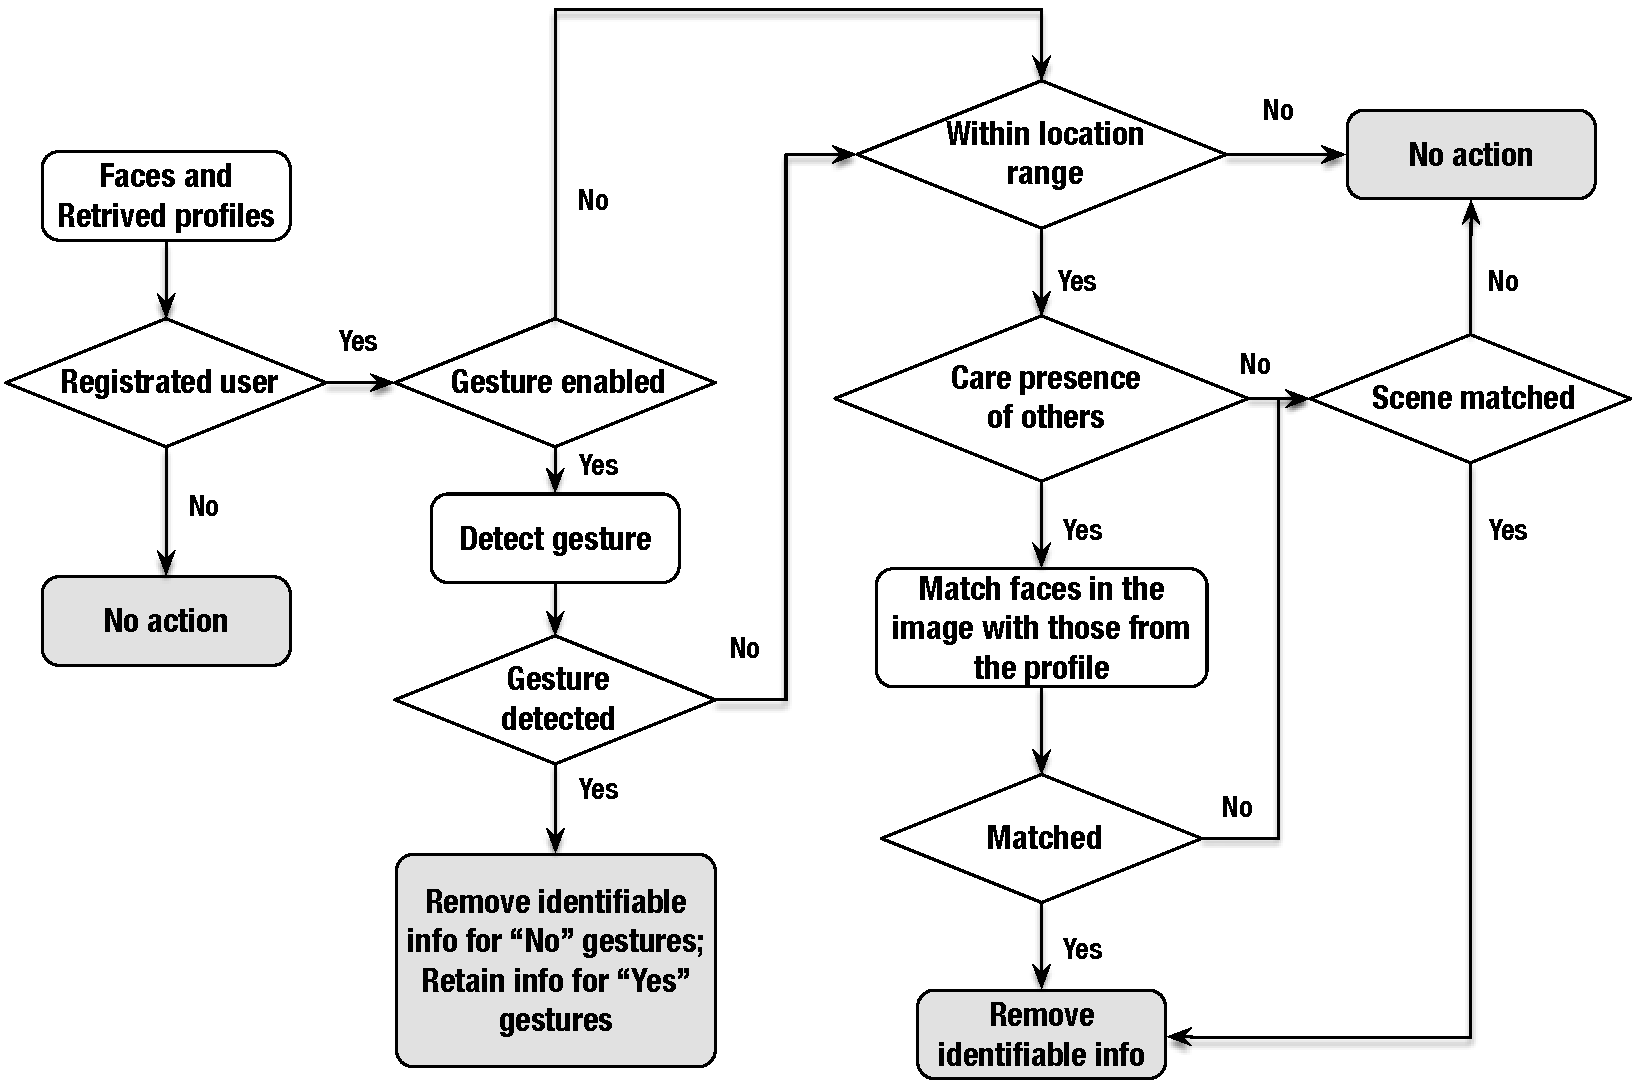
\includegraphics[width=0.6\textwidth]{figure/ch4-decisiontree.pdf}
    \caption{Steps of decisions about actions to be applied on detected faces.}
    \label{fig:ch4-decisiontree}
\end{figure}

  \item[{Decision making:}] Fig~\ref{fig:ch4-decisiontree} gives the detailed decision steps. Note that in this process, we need to match a detected gesture with the right face or people who issued the gesture, currently we simply take the nearest face of a detected gesture as the person who issued this gesture, thus it requires the user to put his hand near his face when sending "yes/no" gestures. As seen from the figure, when the detected face is recognized as a registered user, and context including location, scene, presence of other people and gesture matched with recognized user's profile, this detected face will be removed. For other cases, the face will be kept but it may cause removal of other faces in the face matching step.


  \item[{Concurrent requests:}] To enable concurrent requests from different client apps, we implement multiple "recognition" workers to process the queued messages from all the clients, recognition results from different workers will be collected and put into a result queue, followed by multiple "mailing" workers to make decision masks and mail the decision masks back to corresponding blocked client threads. We tested with a server configuration - "Intel i7-5820K CPU, 16GB RAM, GeForce 980Ti Graphic Card(6GB RAM)" and the campus's Wi-Fi network, the time from start sending message to receive server's response is $1-2s$, depending on the message type. The total time from capturing moment to the enforcement of protection actions is $2-4s$, depending on how many faces detected. Most time is spent on facial feature extraction and message data transmission. Note that processing in the server side is relatively fast, gesture recognition of one image takes $200-300ms$, while the time spent on SVM face classifier and face matching is negligible. With 6GB GPU RAM, the server can serve 3 gesture recognition workers at the same time, supporting 5-10 concurrent requests. The implementation of Cardea is hosted in~\cite{links:cardeaproj}.

\end{description}
% \section{Evaluation}


\newpage

\chapter{Conclusion and Future Work}\label{sec-conclusion}

In this thesis we present Cardea, a visual privacy control service framework that aims to address individual's visual privacy issues caused by pervasive cameras. Users can express their privacy preferences in terms of location, scenes, and presence of others. Furthermore, "Yes" and "No" gestures can be used to temporarily modify users' privacy settings. The combination of context-dependent privacy profiles and interactive instructions provides a flexible and convenient way for individuals to control their visual privacy.



Privacy itself is an abstract concept and can not be hard coded if we are aiming at a smart and general control framework. We believe deep learning methods will be applied more and more on privacy control area, towards the direction of learning visual privacy concerns automatically with bigger and higher quality dataset available in future. Based on Cardea's current design, implementation and evaluation, we propose the following future works for improvement:

\begin{itemize}

\item Recently there are many research works about neural network model compression~\cite{han2015deep}, which points us a straight way to decrease the resources consumption, especially for Android client apps. Managing to deploy neural networks on mobile's GPU will save resources both in terms of RAM usage and computation, this requires Cuda or OpenCL implementation of related layers. Also during the forwarding time, activations of all layers are unnecessarily kept in memory for backpropagation which is not needed in deployment time, an implementation of forwarding phase that only keep previous layer's activation will largely reduce memory consumption, which is very important to mobile devices.
\item The requirement of connection to the server makes Cardea easily hackable. An ad hoc approach that mobile devices broadcast owners' facial features as well as privacy preferences to nearby devices is possible if the RPN layer is implemented in C++, making gesture recognition runs locally. Another advantage of ad hoc solution is there will be no large scale face recognition problem, instead it becomes a small scale face matching/verification problem. We also consider using siamese network for better performance of face matching.
\item Preparing larger and more comprehensive dataset for each task is definitely needed. Both scene classification model and gesture recognition model can benefit a lot if we are able to collect more daily life images with better labels or annotations. How to get supervised signals about visual privacy concerns from the design of user interactions worth investigation, integration of these interactions in life logging devices will provide high quality training dataset.

\end{itemize}



\newpage


%%%%%%%%%%%%%%%%%%%%%%%%%%%%%%%%%%%%%%%%%%%%%%%%%%%%%%%%%%%%%%%%%%%%%%%%%
%                                                                       %
%      9) BIBLIOGRAPHY                                                  %
%                                                                       %
% This example uses bibtex to generate the required Bibliography. Refer %
% to the % the file ustthesis_test.bib for the entries of the           %
% Bibliography. Note that only the cited entries are printed.           %
%                                                                       %
% If BibTeX is not used to typeset the bibliography, replace the        %
% following line with the \begin{thebibliography} and \end{bibliography}%
% commands (the "thebibliography" environment) to process the           %
% Bibliography.                                                         %
%                                                                       %
%%%%%%%%%%%%%%%%%%%%%%%%%%%%%%%%%%%%%%%%%%%%%%%%%%%%%%%%%%%%%%%%%%%%%%%%%

%%%%%%%%%%%%%%%%%%%%%%%%%%%%%%%%%%%%%%%%%%%%%%%%%%%%%%%%%%%%%%%%%%%%%%%%%
%                                                                       %
% The recommended bibliography style is the IEEE bibliography style.    %
% "ustbib" defines the IEEE bibliography standard with the added        %
% ability of sorting the items by name of author.                       %
%                                                                       %
% If you are not using BibTeX to process your Bibliography, comment out %
% the following line.                                                   %
%                                                                       %
%%%%%%%%%%%%%%%%%%%%%%%%%%%%%%%%%%%%%%%%%%%%%%%%%%%%%%%%%%%%%%%%%%%%%%%%%

% if use bibtex
% \bibliographystyle{plain}
% \bibliography{ref}

% if use biber
\printbibliography[heading=bibintoc]

% Please run "bibtex ustthesis_test" before the bibliography can be
% included.

%%%%%%%%%%%%%%%%%%%%%%%%%%%%%%%%%%%%%%%%%%%%%%%%%%%%%%%%%%%%%%%%%%%%%%%%%
%                                                                       %
%     10) APPENDIX (If Any)                                              %
%                                                                       %
% \appendix command marks the beginning of the APPENDIX part of the     %
% Thesis. The usual \chapter command is used for the different chapters %
% of the Appendix.                                                      %
%                                                                       %
%%%%%%%%%%%%%%%%%%%%%%%%%%%%%%%%%%%%%%%%%%%%%%%%%%%%%%%%%%%%%%%%%%%%%%%%%


%%%%%%%%%%%%%%%%%%%%%%%%%%%%%%%%%%%%%%%%%%%%%%%%%%%%%%%%%%%%%%%%%%%%%%%%%
%                                                                       %
%     11) BIOGRAPHY (Optional)                                          %
%                                                                       %
% \biography and \endbiography are used to define the optional          %
% Biography of the author of the Thesis.                                %
%                                                                       %
%%%%%%%%%%%%%%%%%%%%%%%%%%%%%%%%%%%%%%%%%%%%%%%%%%%%%%%%%%%%%%%%%%%%%%%%%

% \biography
% The biography of the student is ALSO optional.
% \endbiography

\end{document}
